\chapter[Resultados]{Resultados}

A partir do estudo e pesquisa realizado até o momento determinamos o que utilizar no conjunto do sistema, levantando um perfil que a equipe acredita ser a mais viável em termos de interação, custo-benefício, tempo, conhecimento técnico e outros fatores importantes para o projeto. Será desenvolvido um kit com capacidade de ser acoplado em diversas cadeiras de rodas afim de facilitar a mobilidade elétrica em cadeiras manuais. Os resultados levantados estão disposto no decorrer do capítulo.

\section{Estrutura}

Com a utilização do programa CATIA V5 3D foi estruturado o sistema acoplado à cadeira de rodas, \ref{fig:vista_isometrica_traseira}. Visando três preceitos básicos: comodidade, acessibilidade e conforto.

\begin{figure}[!htb]
\centering
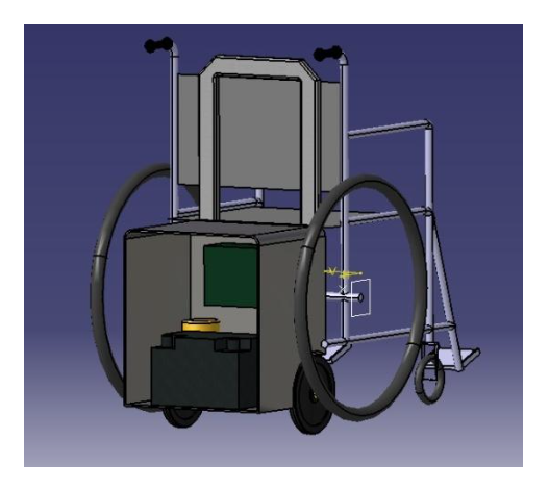
\includegraphics[width=0.5\textwidth]{figuras/estrutura/vista_isometrica_traseira}
\caption{Vista Isométrica Traseira}
\label{fig:vista_isometrica_traseira}
\end{figure}

O objetivo do projeto é desenvolver uma estrutura de fácil conexão e resistente. O produto proposto, ver figura \ref{fig:traseira}, \ref{fig:sistema}, \ref{fig:lateral} e \ref{fig:superior},deve-se acoplar a qualquer cadeira de rodas.

Foi pensado em um dispositivo no formato de uma mala para que seja de fácil conexão, uso e manuseio.

\begin{figure}[!htb]
\centering
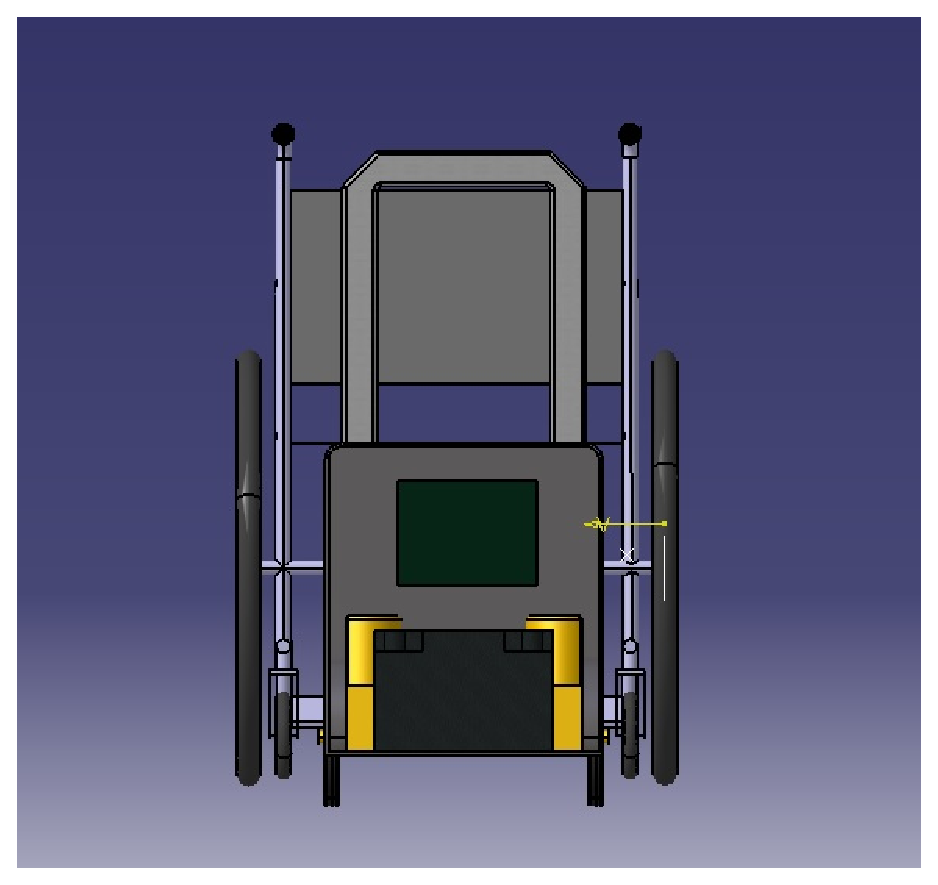
\includegraphics[width=0.5\textwidth]{figuras/estrutura/vista_traseira}
\caption{Vista Traseira}
\label{fig:traseira}
\end{figure}

A forma como a mala será acoplada a cadeira usa como base as hastes da mala e as hastes verticais aonde as manoplas utilizadas para empurrar manualmente a cadeira são fixadas. Tendo em vista que são rígidas e normatizadas pela NBR 9050 as hastes verticais da cadeira tem a distancia e espessura já definidas, o que facilita o desenvolvimento de um produto que possa ser usado em qualquer cadeira de rodas que esteja dentro dos padrões impostos pela norma.

\begin{figure}[!htb]
\centering
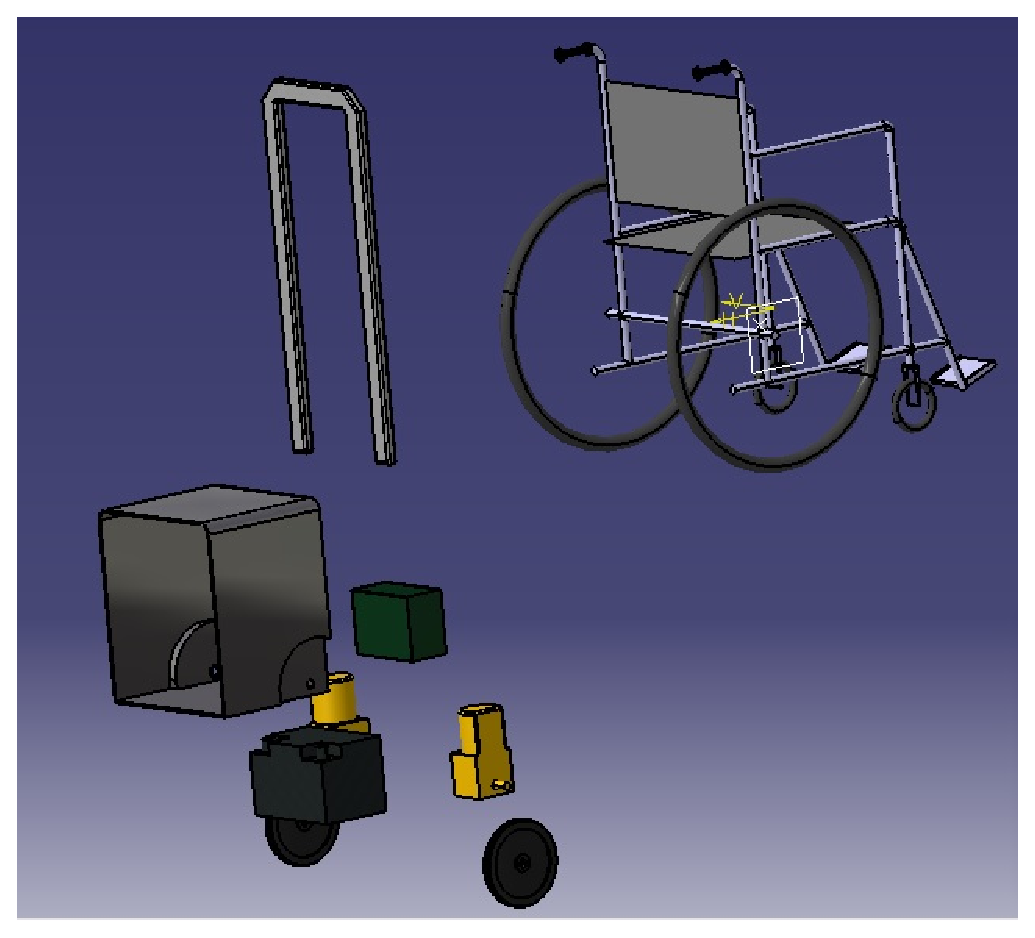
\includegraphics[width=0.5\textwidth]{figuras/estrutura/explode}
\caption{Visão do Sistema}
\label{fig:sistema}
\end{figure}

Cada roda possuirá um motor próprio para que seja possível rotaciona-lás em sentidos opostos, por exemplo, quando for necessário fazer manobras em que a rotação deve ocorre em torno do eixo do próprio cadeirante, movimento muito comum para manobrar uma cadeira de rodas. Assim o cadeirante se sentira confortável e não terá grandes dificuldades quando for manobrar a cadeira, já que a lógica de controle será a mesma usada quando se propulsiona manualmente a cadeira.

\begin{figure}[!htb]
\centering
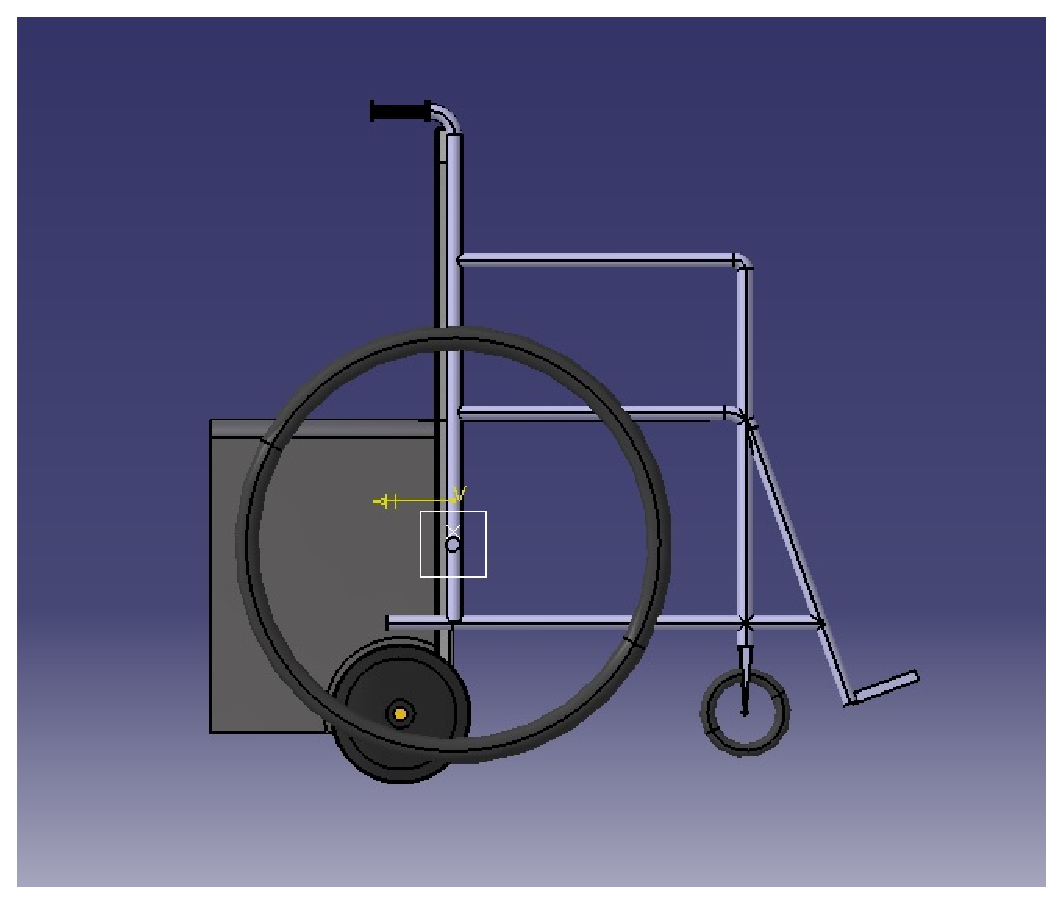
\includegraphics[width=0.5\textwidth]{figuras/estrutura/vista_lateral_cadeira}
\caption{Imagem Lateral}
\label{fig:lateral}
\end{figure}

Como pode se notar nas figuras, o sistema de propulsão devera empurrar a cadeira de rodas, pois assim podemos aproximar o máximo possível o eixo da roda que ira gerar o movimento ao eixo da maior roda da cadeira, o que diminui a quantidade de torque necessário para movimentar o conjunto, fazendo com que o consumo de energia diminua e possibilite o uso de um motor de menor potencia, que diminuirá o custo do produto final.

\begin{figure}[!htb]
\centering
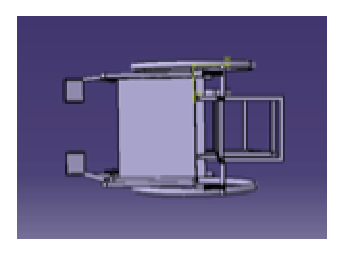
\includegraphics[width=0.5\textwidth]{figuras/estrutura/vista_superior}
\caption{Imagem Superior}
\label{fig:superior}
\end{figure}

\subsection{Protótipo}

A partir do policloreto de vinila, usualmente conhecido como PVC, foi feita uma estrutura de teste para encaixar na parte de trás da cadeira de rodas, com o intuito de buscar a melhor regulação to tamanho da estrutura. O protótipo em questão foi feito para se chegar o mais próximo de um modelo ideal capaz de se acoplar as cadeiras regulamentadas pela NBR 9050.

O protótipo é uma estrutura retangular com uma alça de regulação de largura, seguido de dois “joelhos” em PVC para o acoplamento das rodinhas e da haste, dois encaixes com três saídas para regulação da barra de encaixe superior da cadeira. Há quatro furos na barra de regulação de largura, a qual serve para se adequar ao tipo de cadeira de rodas sendo utilizada, vide figura para mais detalhes \ref{fig:acoplamento}.

\begin{figure}[!htb]
\centering
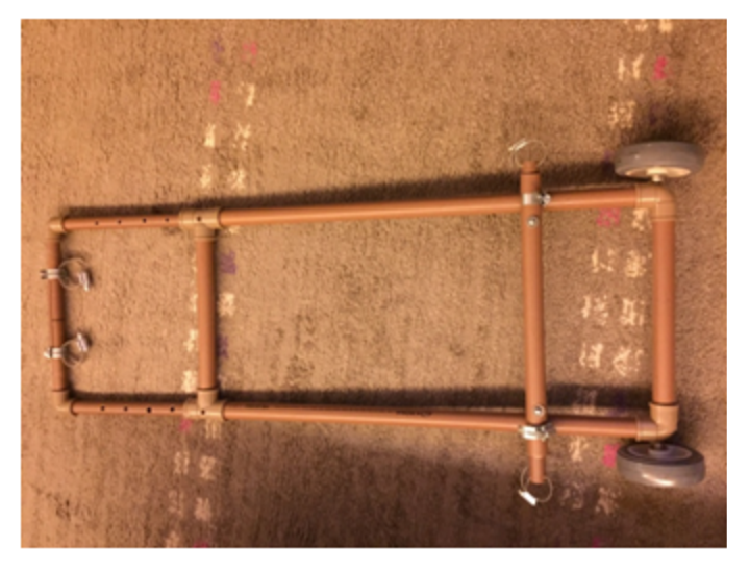
\includegraphics[width=0.7\textwidth]{figuras/resultados/acoplamento}
\caption{Estrutura de acoplamento}
\label{fig:acoplamento}
\end{figure}

No protótipo alguns mecanismos de acoplamento foram testados afim de garantir o encaixe mais prático e eficiente do sistema com a cadeira. Dentre as tentativas, foram utilizados materiais como: velcro, correias de nylon e braçadeiras utilizadas em construção civil, que foi a solução mais bem-sucedida. Estas podem ser observadas nas extremidades de acoplamento do sistema na \ref{fig:acoplamento}. Este mecanismo foi posteriormente substituído no acoplamento superior do mecanismo por um sistema  \ref{fig:acop_bracadeira} de funcionamento análogo, porém, de estrutura mais robusta, que foi fabricado pela própria equipe.

\begin{figure}[!htb]
\centering
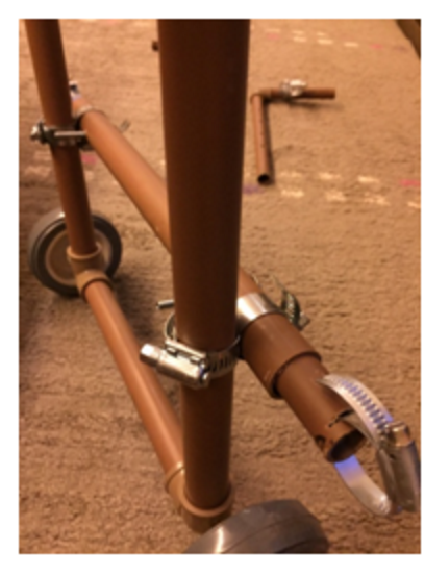
\includegraphics[width=0.4\textwidth]{figuras/resultados/acop_bracadeira}
\caption{Sistema de acoplamento com braçadeira}
\label{fig:acop_bracadeira}
\end{figure}

Na parte da estrutura mostrada na figura \ref{fig:acop_bracadeira} existem dois “joelhos” que ligam as rodinhas com o as barras de PVC, além de uma barra em paralelo com a barra das rodinhas, capaz de variar em altura e largura para se adequar ao tamanho da cadeira utilizada, e  duas braçadeiras nas pontas das barras que irão se acoplar a cadeira de rodas.

\begin{figure}[!htb]
\centering
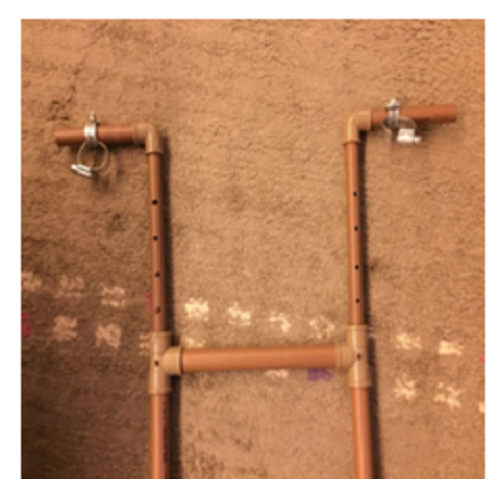
\includegraphics[width=0.5\textwidth]{figuras/resultados/superior_estrutura}
\caption{Parte superior da estrutura}
\label{fig:superior_estrutura}
\end{figure}

A figura \ref{fig:superior_estrutura} representa a parte superior da estrutura, ela contem dois ''joelhos'' capazes de ligar as duas alças com as duas barras de sustentação da estrutura. Há dois ''T'' com furo que ligam três barras de cada lado, eles tem a função de regular a altura com o seis furos nas barras de movimentação. Na alça estão duas braçadeiras livres, que se ligam na parte superior da cadeira de rodas, assim como a parte superior já descrita.

Os componentes utilizados para se fazer este modelo são descritos:
\begin{itemize}
  \item Oito braçadeiras circulares de curso infinito;
  \item Quarto ''joelhos'' de 90$^\circ$;
  \item Dois ''T'';
  \item Duas rodas;
  \item Barras de PVC com diâmetros de 20mm e 25mm;
  \item Quatro parafusos;
  \item Oito arruelas;
  \item Quatro porcas.
\end{itemize}

O protótipo apresentado na figura \ref{fig:estr_prototipo} foi capaz de mostrar como funcionará o sistema, e todo encaixe necessário para não ocorrer folga e desconforto ao cadeirante. Esta estrutura se assemelha com as medidas do sistema original, mudando apenas o material da execução e do funcionamento. Obteve-se excelentes resultados testando tal protótipo em dois modelos de cadeira de rodas.

\begin{figure}[!htb]
\centering
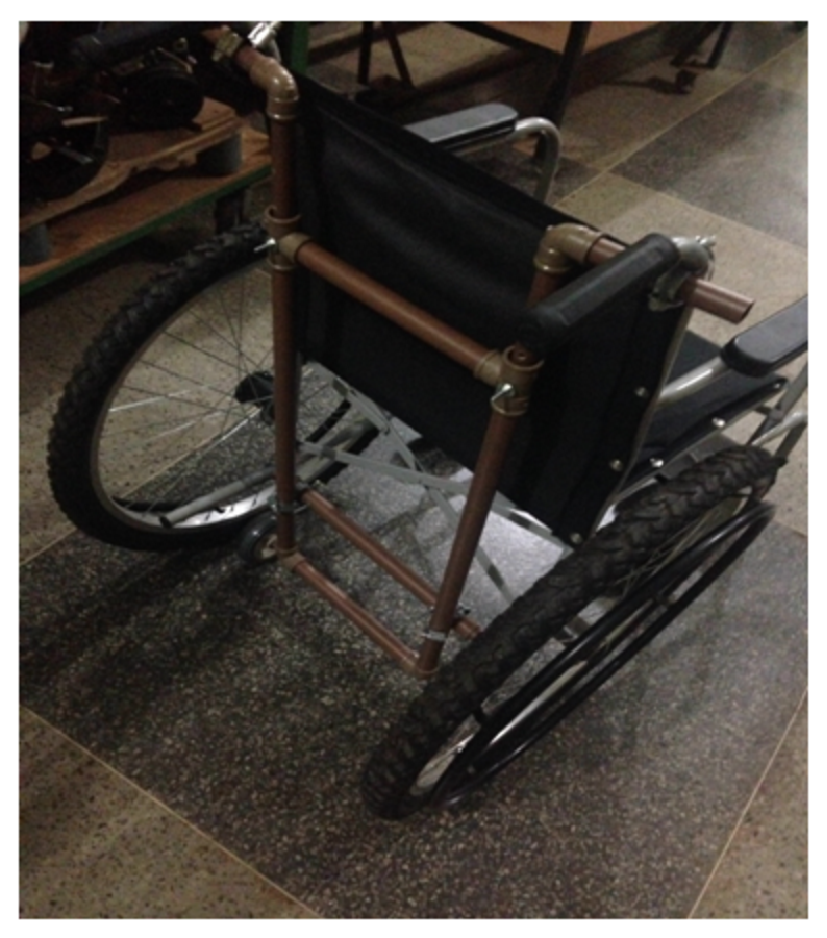
\includegraphics[width=0.4\textwidth]{figuras/resultados/estr_prototipo}
\caption{Estrutura acoplada a cadeira}
\label{fig:estr_prototipo}
\end{figure}

A etapa seguinte foi a definição do material a ser utilizado no produto final. A melhor opção encontrada foi o aço SAE 1020, por atender todos os requisitos com consideráveis vantagens quando comparados a alternativas como ferro ou alumínio.

Um modelo 3D do projeto foi desenvolvido utilizando o software CATIA V5R19, que já considerou o Aço 1020 em seções quadradas de 20 e 18 mm assim como redondas de 18 mm para as alças superiores. A partir do deste modelo, foi possível proceder com a montagem do mecanismos com toda base necessária para medidas, cortes, junções e elementos de todo o produto. Posteriormente, também foi possível uma análise estrutural.

Alguns elementos foram modificados no sistema de acoplamento inferior e superior, em relação ao que foi apresentado no ponto de controle 2 para que houvesse maior aderência do dispositivo à cadeira de rodas, e evitar esforços mecânicos indesejáveis. Como mostra a \ref{fig:furos_estrutura}, na parte inferior do dispositivo foram adicionados novos furos na vertical, para que a estrutura melhor acople nas cadeiras de rodas de acordo com a NBR 9050.

\begin{figure}[!htb]
\centering
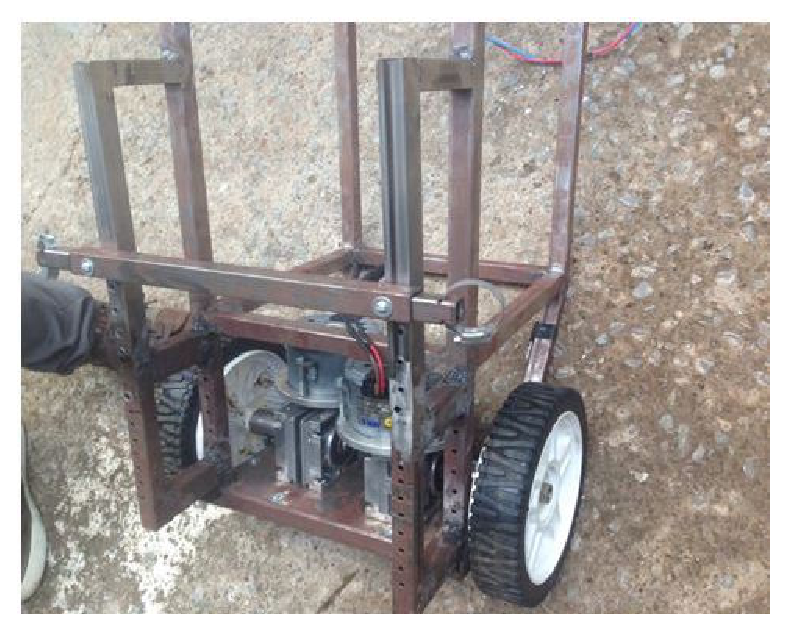
\includegraphics[width=0.55\textwidth]{figuras/resultados/furos_estrutura}
\caption{Novos furos na parte inferior da estrutura}
\label{fig:furos_estrutura}
\end{figure}

A parte superior da estrutura, que recebeu um novo método de acoplamento a cadeira de rodas, através da utilização de tubos de aço, onde a parte inferior de um dos tubos foi soldado transversalmente com a parte superior do outro tubo. Dois parafusos do tipo borboleta foram adicionados na parte central destes tubos para facilitar seu aperto. Um parafuso foi acoplado na parte inferior do tubo inferior, e outro parafuso foi acoplado na parte superior do tubo superior. Esses parafusos, quando apertados, acoplam-se à estrutura da cadeira de rodas de forma mais simplificada, rápida e segura em relação às braçadeiras utilizadas anteriormente. A \ref{fig:novo_acoplamento_superior} abaixo apresenta as mudanças descritas.

\begin{figure}[!htb]
\centering
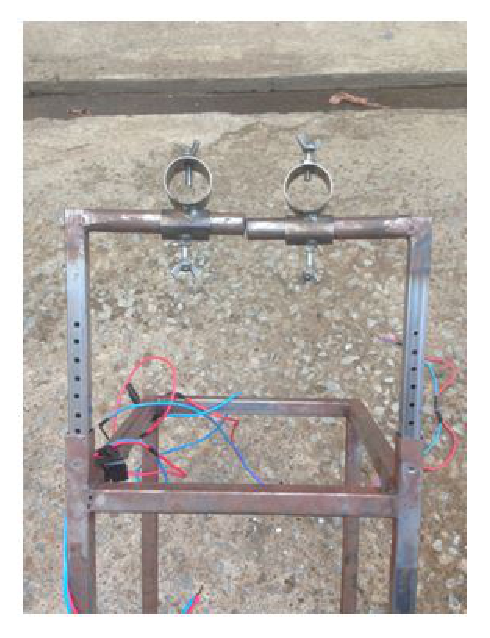
\includegraphics[width=0.4\textwidth]{figuras/resultados/novo_acoplamento_superior}
\caption{Novo acoplamento superior}
\label{fig:novo_acoplamento_superior}
\end{figure}

Com esse novo acoplamento, a parte superior da estrutura pode variar horizontalmente de forma mais simples, já que os tubos inferiores movem-se para a direita e para a esquerda nos braços da estrutura, permitindo um amplo acoplamento em diferentes tipos de cadeiras de rodas.

A figura \ref{fig:esquematico_estr_acoplada} mostra um esquema de como será acoplada a estrutura com a cadeira de rodas, que é feita de maneira simples e rápida. Esta estrutura não interfere no conforto do cadeirante, já que o sistema não interfere na acomodação do cadeirante na cadeira de rodas, enquanto a estrutura não o toca em nenhum momento.

\begin{figure}[!htb]
\centering
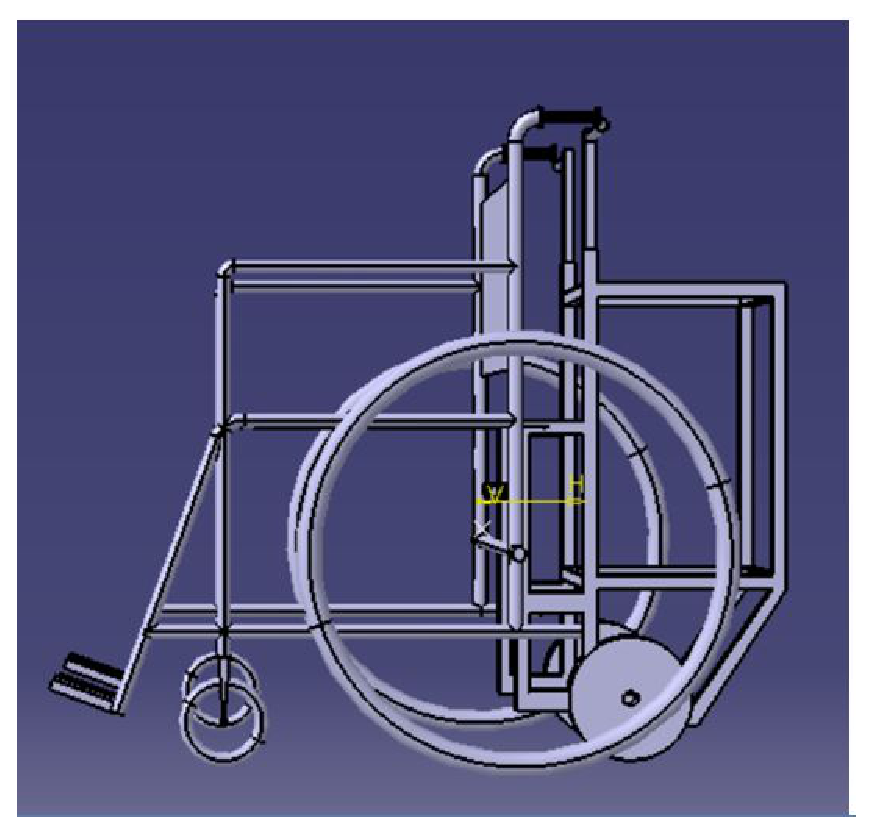
\includegraphics[width=0.5\textwidth]{figuras/resultados/esquematico_estr_acoplada}
\caption{Esquemático de estruturas acopladas}
\label{fig:esquematico_estr_acoplada}
\end{figure}

 \subsection{Esforços Estruturais}

A partir da modelagem tridimensional da estrutura, podem ser demonstradas as tensões segundo o critério de Von Mises, que nos permite ver a tensão de cisalhamento máxima ou a energia de distorção máxima suportada pela estrutura.

\begin{figure}[!htb]
\centering
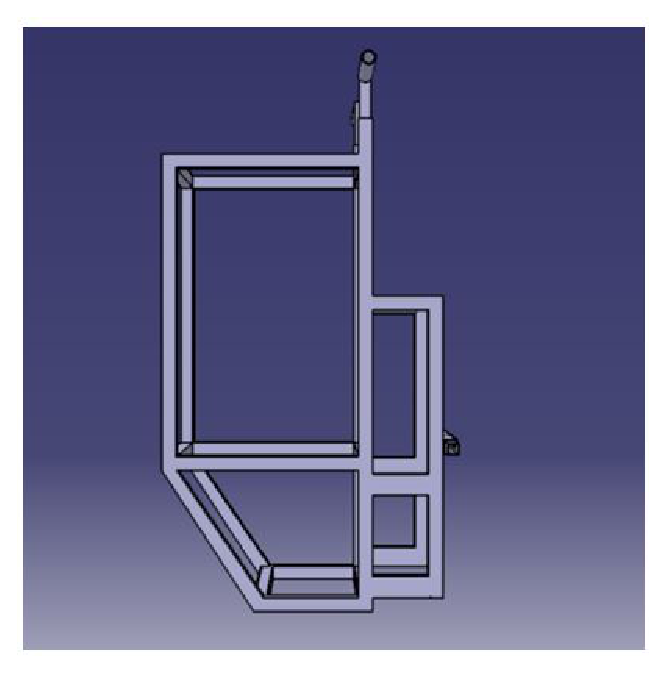
\includegraphics[width=0.5\textwidth]{figuras/resultados/vista_lateral_estrutura}
\caption{Vista Lateral da estrutura do Sistema}
\label{fig:vista_lateral_estrutura}
\end{figure}

A \ref{fig:vista_lateral_estrutura} representa a estrutura vista lateralmente, mostrando todos os compartimentos internos dos motores, bateria e controle. Na parte inferior da estrutura, ficarão os motoredutores, onde deles saem os eixos que se ligam às rodas. Na parte intermediária ficará a bateria, e acima dela, a parte de controle. A inclinação observada na parte inferior esquerda da figura acima foi feita para evitar que a estrutura arraste no chão quando o cadeirante passar por terrenos inclinados como, por exemplo, uma rampa.

\begin{figure}[!htb]
\centering
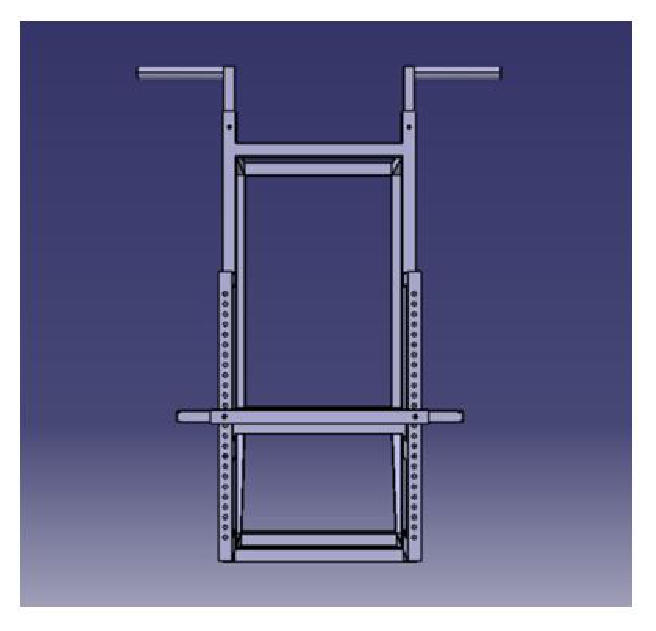
\includegraphics[width=0.5\textwidth]{figuras/resultados/vista_frontal_estrutura}
\caption{Vista frontal da estrutura do Sistema}
\label{fig:vista_frontal_estrutura}
\end{figure}


A \ref{fig:vista_frontal_estrutura} apresenta a parte frontal da estrutura, que será acoplada na parte de trás da cadeira de rodas. Apresentam-se aqui os novos furos que foram feitos na parte inferior, permitindo que o acoplamento inferior se mova em mais posições na vertical. Isto faz com que a estrutura obedeça melhor a NBR 9050. Os braços superiores podem ser, quando necessário, retirados e colocados novamente virados para dentro, formando assim uma espécie de alça para que a estrutura seja puxada ou transportada mais facilmente.

\begin{figure}[!htb]
\centering
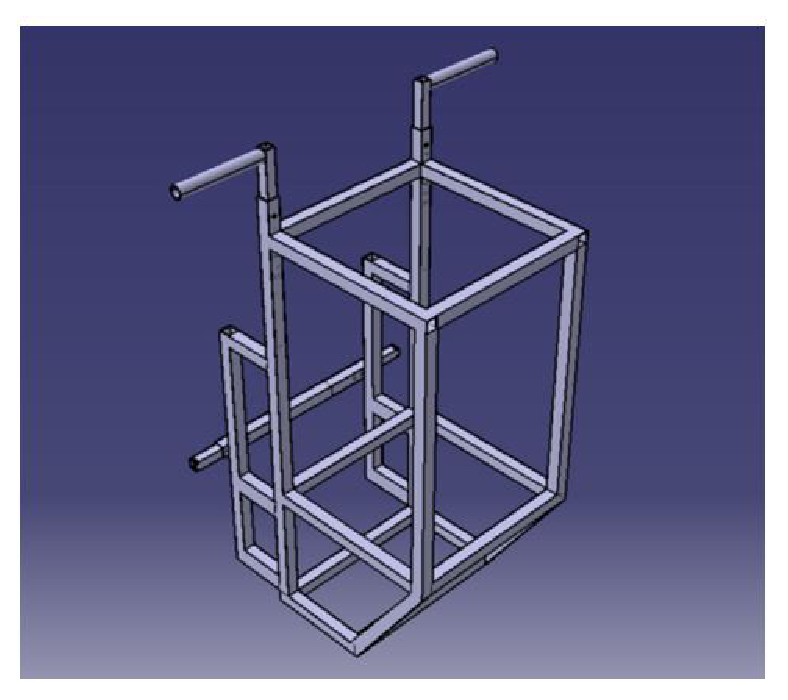
\includegraphics[width=0.5\textwidth]{figuras/resultados/vista_perspectiva_estrutura}
\caption{Vista em perspectiva da estrutura do Sistema}
\label{fig:vista_perspectiva_estrutura}
\end{figure}

Uma visão geral da estrutura é apresentada pela \ref{fig:vista_perspectiva_estrutura}. Aqui observa-se os níveis internos da estrutura, onde ficarão os motores, a bateria e a parte de controle. Além dos braços superiores, que podem se mover em diferentes níveis na vertical para se encaixar melhor na cadeira de rodas, e a parte inferior, também podendo se mover em diferentes níveis na vertical, acoplando facilmente na parte inferior da cadeira de rodas.

\begin{figure}[!ht]
  \subfloat[]{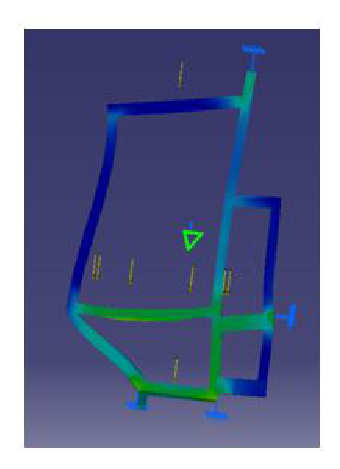
\includegraphics[width = 0.37\textwidth]{figuras/resultados/von_mises_lateral}
   \label{fig:analise_von_mises_1}}
   \subfloat[]{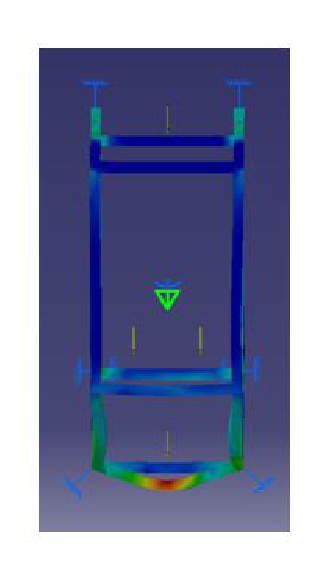
\includegraphics[width = 0.3\textwidth]{figuras/resultados/von_mises_frontal}
   \label{fig:analise_von_mises_2}}
   \subfloat[]{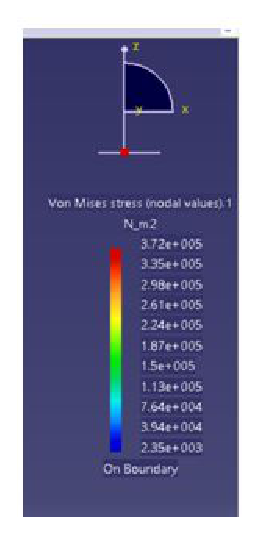
\includegraphics[width = 0.24\textwidth]{figuras/resultados/von_mises_escala}
   \label{fig:analise_von_mises_3}}
  \caption{Tensão de Von Mises máxima e mínima do material}\label{fig:analise_von_mises}
\end{figure}

A figura \ref{fig:analise_von_mises} representa as deformações na estrutura devido aos carregamentos estáticos no sistema e as devidas restrições relativas ao acoplamento e ao contato das rodas com o chão. Os carregamentos adotados foram de 14 kg da bateira, 15 kg dos dois motores e estimados 2 kg de todo o sistema de controle e foram devidamente posicionados em suas posições de trabalho. Vale ressaltar que as deformações apresentadas possuem um fator de aumento de 1000 para possibilitar a visualização. As tensões encontradas no sistema obedeceram o critério de Von Mises, que nos permite notar que a parte inferior da base é o gargalo, pois ela sofre as maiores tensões da estrutura. Na figura (a) verifica-se que a tensão máxima do material é 0.372 MPa, enquanto a figura (b) apresenta a visão frontal destas tensões. Com esses valores sabemos que a estrutura resistirá aos carregamentos a ela submetidos, já que a tensão de escoamento do aço 1020 é de 210Mpa

\subsection{Centro de Massa}

O Cálculo do centro de massa do conjunto total (cadeira, cadeirante e Sistema de automação) foi necessário para o cálculo da potência requerida dos motores. O centro de massa foi estimado a partir da soma vetorial dos centros de massa parciais do conjunto cadeira-cadeirante que foi obtido a partir dos estudos de \cite{artigo_centro_massa}, vide figura \ref{fig:centro_massa_cadeirante}.

\begin{figure}[!htb]
\centering
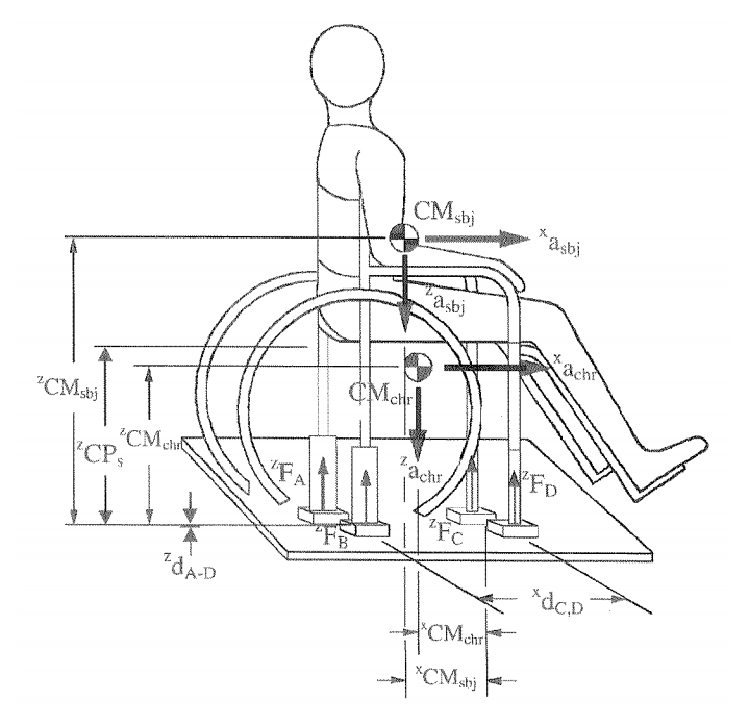
\includegraphics[width = 0.5\textwidth]{figuras/resultados/centro_massa_cadeirante}
\caption{Esquemático posicionamento do centro de massa sistema cadeira e cadeirante. Fonte:\cite{artigo_centro_massa}}
\label{fig:centro_massa_cadeirante}
\end{figure}

O centro de massa do Sistema de automação, vide figura \ref{fig:centro_massa_sistema_automocao}, foi obtido a partir de uma simulação estática da estrutura em que se aplicou os devidos carregamentos e restrições de trabalho.

\begin{figure}[!htb]
\centering
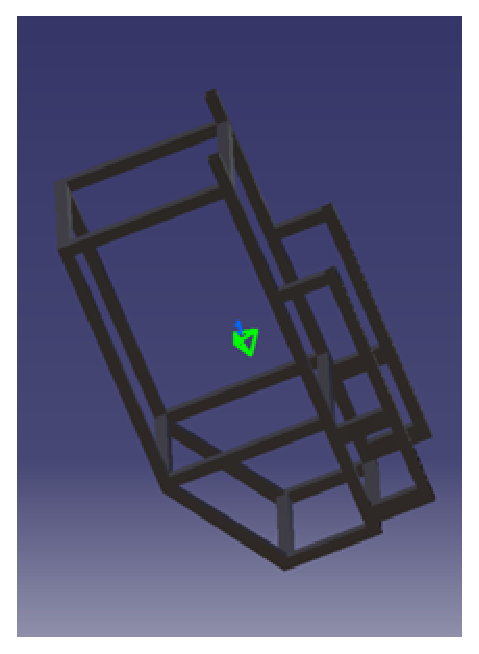
\includegraphics[width = 0.5\textwidth]{figuras/resultados/centro_massa_sistema_automocao}
\caption{Representação do centro de massa do sistema de automação}
\label{fig:centro_massa_sistema_automocao}
\end{figure}

As coordenadas encontradas, tanto na literatura quanto computacionalmente, foram manualmente modificadas de modo a ter o eixo da roda maior da cadeira de rodas como ponto de origem para o cálculo vetorial. Vale lembrar que os cálculos desconsideram possíveis deformidades no corpo do usuário que possam causar assimetria na distribuição de massa.

Desta maneira, os cálculos resultaram que o centro de massa está, portanto, a 45 cm do eixo das rodas maiores da cadeira verticalmente para cima, e a 5 cm deste eixo horizontalmente na direçao do usuário. Foi observado que o centro de massa foi deslocado para mais perto do eixo das rodas maiores por causa de sua carga adicional ao sistema.

\section{Power-Train}

\subsection[Resistência a Rolagem]{Resistência a Rolagem}

Ao acoplar o protótipo criado para automatizar a cadeira de rodas, acrescenta-se um peso a mais ao sistema, assim como um ponto a mais de contato de distribuição da massa total é adicionado ao sistema. Desta maneira, as forças nas rodas traseiras são aliviadas por serem divididas com as rodas do protótipo. A figura \ref{fig:finalmente_essa_imagem} abaixo apresenta as distâncias entre os eixos das rodas da cadeira e do protótipo ao centro de massa.

\begin{figure}[!htb]
	\centering
	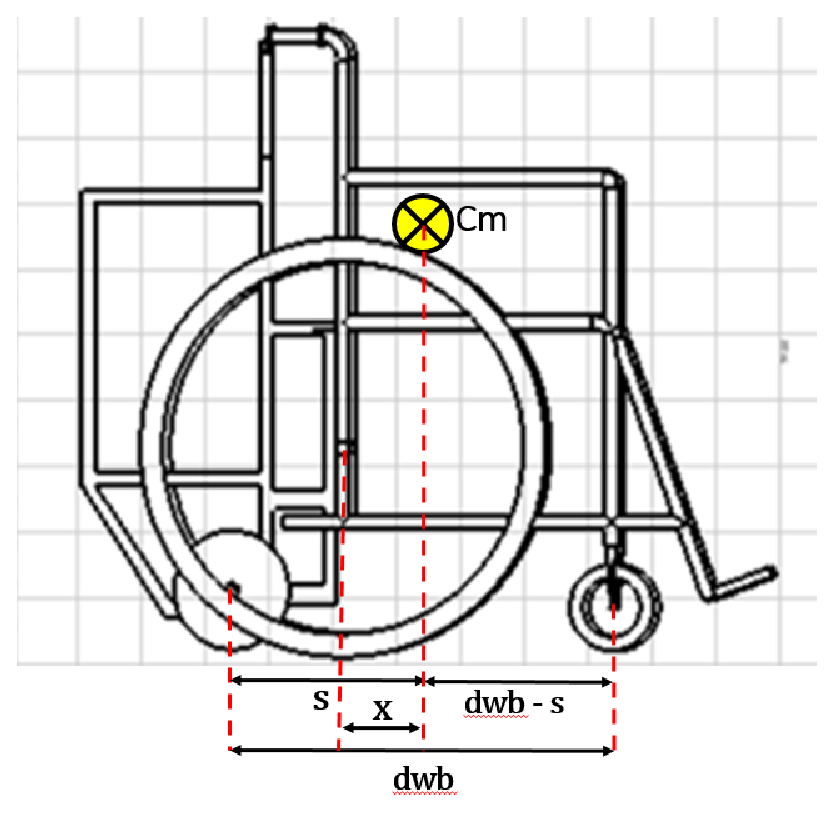
\includegraphics[width = 0.5\textwidth]{figuras/resultados/finalmente_essa_imagem}
	\caption{Diagrama das Variáveis para determinação da Resistência de Rolagem com o protótipo acoplado. Autoria própria.}
	\label{fig:finalmente_essa_imagem}
\end{figure}

Desta maneira, as equações discutidas anteriormente são modificadas abaixo para se ajustarem ao protótipo acoplado, onde $s$ é a distância entre as rodas do protótipo e o centro de massa, e \textit{dwb} é a distância entre o eixo das rodas dianteiras e as rodas do protótipo. Como explicado na seção anterior, a distância entre o eixo das rodas maiores e o centro de massa, neste caso $x$, foi igual a 5 cm.

\begin{equation}
	f_p=m*g\frac{(dwb-s-x)}{dwb} ; f_{p,rr}=\mu*f_p
\end{equation}
\begin{equation}
	f_r=m*g\frac{(dwb-s)}{dwb} ; f_{r,rr}=\mu*f_r
\end{equation}
\begin{equation}
	f_c=m*g\frac{x}{dwb} ; f_{c,rr}=\mu*f_c
\end{equation}
\begin{equation}
	f_{rr}=f_{c,rr}+f_{r,rr}+f_{p,rr}
\end{equation}

A distribuiçao do peso na cadeira de rodas é, portanto, de 44.4 \%\ para a roda do sistema, 51.4 \% para as rodas traseiras da cadeira e 4.2 \%\ para as rodas dianteiras da cadeira. As constantes usadas nestes cálculos foram:

As constantes usadas nestes cálculos foram:


\begin{itemize}
	\item $\mu$ = 0.03. Coeficiente estimado para o pior piso e pior tipo de material da roda \cite{rolling_resistance};
	\item m = 150 kg (massa máxima);
	\item g = 9.81 $m/s^2$;
	\item dwb = 72 cm;
	\item s = 35 cm;
	\item x = 5 cm;
\end{itemize}

Os resultados das forças de resistência ao rolamento são, portanto:

\begin{itemize}
	\item fp,rr = 19.62 N;
	\item fr,rr = 22.686 N;
	\item fc,rr = 1.839 N;
	\item frr = 44.145 N;
\end{itemize}

Esta força deve ser vencida pelos motores acoplados ao protótipo de modo a retirar a cadeira da inércia quando todas as rodas da cadeira estão alinhadas para frente perfeitamente. Porém, isto nem sempre acontece.

Portanto foi feita uma simulação para quando as rodas dianteiras estão paralelas às rodas traseiras. Nesta configuração, as rodas dianteiras fornecem uma resistência a mais ao movimento. Esta resistência foi considerada como uma resistência de atrito estático e depende do coeficiente de atrito estático do material das rodas dianteiras ($\mu e$) e da fração da massa suportada nas rodas dianteiras que pode ser definida como:

\begin{equation}
c = \frac{x}{dwb}
\end{equation}

A resistência adicional pode ser definida, portanto, como:

\begin{equation}
f_{ce}= m*g* \mu_e \frac{x}{dwb}
\end{equation}

A resistência total ao movimento (fT) seria portanto a soma das resistências de rolamento com a de atrito estático:

\begin{equation}
f_T = f_{rr} + f_{ce} = 44.146+45.984 = 90.129 N
\end{equation}

Isto exige um torque inicial de 9.0129 Nm (dado que os raios das rodas do protótipo são de 10 cm). Portanto, pode-se dizer que, nesta situação, a potência necessária para retirar a cadeira da inércia é de:

\begin{equation}
P = T*\omega = 9.0129*26.18 = 235.96 W
\end{equation}

  A potência entregue pelos motores à cadeira de rodas será maior que estes 235.96 W . A diferença entre a entregue e a necessária para retirar a cadeira da inércia será considerável, o que poderia causar um arranque repentino do sistema. Este tranco poderia prejudicar o usuário assim como a cadeira. A solução para este problema está no uso de pontes H, que fornecem corrente aos motores de forma gradativa a medida que o usuário empurra o joystick, diminuindo o arranque do protótipo.

  \subsection{Moto-redutor}

  Será utilizado no projeto o motor de corrente contínua. A escolha foi feita pois esse tipo de motor é muito utilizado em projetos que necessitam de velocidades variáveis, eles também apresentam uma região de torque e potência constante e são simples de realizar a aceleração e a desaceleração \cite{manual_bateria_unipower}.

  Após uma vasta pesquisa no mercado de motores e redutores, optou-se por comprar dois moto-redutores feitos pela empresa MKS Redutores de São Paulo. O motor com redutor escolhido para o projeto foi o MR com motor GPB que possui as seguintes especificações:

  \begin{itemize}
    \item Potência de 305 a 350 W;
    \item 12 ou 24 Vcc;
    \item Rotação de entrada de 2500 rpm;
    \item Reduções de 1:10 até 1:60.
  \end{itemize}

  Especificações a serem atendidas:

  \begin{itemize}
    \item Velocidade máxima de 10 km/h;
    \item 12 Volts corrente contínua;
    \item Peso da bateria 15 kg;
    \item Peso da cadeira (valor aproximado) 15kg;
    \item Peso total estimado: 150 Kg;
    \item Redução de pelo menos 1:10.
  \end{itemize}

  \subsection{Bateria}

  A bateria de chumbo-ácido é muito utilizada hoje em dia em diferentes áreas, como automóveis, sistemas de fornecimento de energia elétrica ininterrupta (no-breaks) e cadeiras de rodas elétricas. Desprezando-se o problema do peso e considerando as observações feitas anteriormente no capítulo \ref{cap:fundamentacao_teorica}, a bateria de chumbo-ácido selada foi a escolhida para o projeto, considerando ainda o seu fácil acesso no mercado e baixo custo.

  \subsubsection{Autonomia}

  Segundo a literatura, cadeiras de rodas elétricas trabalham com motores de corrente contínua entre 250 W a 300 W de potência. Há diversas maneiras de chegar neste valor, como por distribuição de forças, por balanço de energia, por forças em um plano inclinado, entre outras. Para este projeto fez-se uma estimativa da potência necessária através do balanço de energia \cite{acionamento_motores_cadeira}.

  A energia fornecida pelo motor deve ser igual à energia cinética da cadeira. Sendo a massa máxima que a cadeira de rodas aguenta de 150 kg e considerando que cadeiras de rodas elétricas chegam até 10 km/h, tem-se:


  \begin{equation}
    Em = \frac{m*V^2}{2}
  \end{equation}

  Onde $Em$ é a energia fornecida pelo motor, $m$ é a massa de 150 kg e $V$ é a velocidade de 2.77 m/s. Assim, a energia necessária para mover a cadeira é de 578.7 J. Sendo 1 Watt igual a 1 J/s, tem-se, portanto, 578.7 W.

  Após uma pesquisa no mercado, foram adquiridos dois motores de corrente contínua de 12 Volts e 305 Watts para o projeto, assim, a potência total entregue ao sistema é de 610 W. Este tipo de motor possui perdas de potência tanto mecânicas (\textit{Pm}) quanto térmicas (\textit{Pj}) \cite{perdas}. A primeira está associada a perdas por causa da velocidade: por atrito, nas escovas do motor e por curto-circuito; estima-se que estas juntas sejam cerca de 3 a 5\% da potência nominal do motor.

  As perdas térmicas estão associadas ao efeito Joule: os fios usados nos enrolamentos dos motores apresentam certa resistência elétrica. A corrente entregue para o motor, em máxima potência é dada pela divisão da potência pela tensão do motor: \textit{I} = 25.417 A. Desta forma, a resistência \textit{R} pode ser calculada pela fórmula da potência a seguir:

  \begin{equation}
  P = R*I, assim, R = \frac{305}{25.417^2} = 0.47231 \ohm
  \end{equation}

  As perdas nos enrolamentos (Pj) é portanto:

  \begin{equation}
  Pj = R*I = 0.47213*25.417 = 12 W
  \end{equation}

  As perdas totais (Pt) são, portanto:

  \begin{equation}
  Pt = Pj+Pm = 12+(305*0.05) = 27.25 W
  \end{equation}

  Estas perdas representam cerca de 9\% da potência nominal do motor. Desta maneira, se deve adicionar um termo de perdas a serem superadas pelos motores à equação da energia, este termo $\epsilon$ seria igual a 1.09:

  \begin{equation}
    Em = \frac{m*V^2*\epsilon}{2}
  \end{equation}

  Assim, a energia necessária para mover a estrutura seria de 630.434 J, ou 630.434 W de potência. Para encontrar o valor da velocidade final do sistema é preciso rearranjar a equação acima. Uma eficiência de 80\% foi atribuída ao acoplamento das rodas com o eixo do motor. Estes 20\% englobam as perdas no redutor, perdas por escorregamento da conexão do redutor e da roda com o chão, entre outros. Assim, temos:

  \begin{equation}
  Em = 0.8*\sqrt{\frac{600*2}{m*\epsilon}}
  \end{equation}

  Assim, a estimativa da velocidade máxima que a cadeira deve obter será de aproximadamente 8.6 km/h, que é uma velocidade bem razoável para este tipo de sistema. Sabe-se que a velocidade angular é dada pela divisão da velocidade linear pelo raio:

  \begin{equation}
  \omega = \frac{V}{r}
  \end{equation}

  Logo, utilizando a velocidade estimada acima, a velocidade angular obtida é de 23.9 rad/s ou 228.31 rpm. Considerando as especificações do motor, sua velocidade angular nominal de 2500 rpm, teria de ser feita uma redução de pelo menos 1:11, onde a velocidade angular de saída do redutor seria de 227.3 rpm.

  Por motivos construtivos do motoredutor, a redução só pode ser feita de 1:10 ou de 1:15. Desta forma optou-se por uma redução de 1:10, que proporciona velocidade de saída nominal de 250 rpm (26.18 rad/s) no redutor. Sendo o torque a divisão da potência pela velocidade angular, o torque gerado é de 23.30 Nm.

  Para atender dois motores de 305 W, será conectada uma bateria de carro de chumbo-ácido selado de 12 V (U) e capacidade de 60Ah (I*$\Delta$t), tem-se que a energia $E$ gerada pela bateria é de:

  \begin{equation}
  E = (I*\Delta t)*U = (60Ah)*12 = 720Wh
  \end{equation}

  Desta forma, considerando a potência consumida pelos dispositivos eletrônicos de controle desprezível, tem-se que a autonomia da bateria seria de pouco mais de uma hora:

  \begin{equation}
  \Delta t = \frac{720 Wh}{610 W} = 1.18 h = 1 hora e 10 minutos
  \end{equation}

\section{Controle}

  O controle da cadeira de rodas será feito utilizando 3 módulos: Joystick, Controlador central e Motor.
  O módulo Joystick, para receber os comandos provenientes do usuário e enviar estes comando para o controlador central. O módulo do controlador central, recebe as informações do módulo anterior, as processa e faz o envio para o módulo Motor. O módulo Motor recebe as informações enviadas pelo módulo do controlador central, produzindo 2 pulsos de PWM e enviando-os para as pontes H, com o intuito de controlar a intensidade e direção dos motores.

\subsection{Atual Panorama}

  O módulo Controlador central possui um Raspberry, utilizado para processar as informações submetidas a ele pelo módulo Joystick, e enviar as informações processadas para o módulo Motor. Isto é possivel graças ao software implementado. Nesta implementação foi utilizada o protocolo de comunicação UART.

  A primeira versão deste software foi feita de forma sequencial: era feita a recepção dos dados provenientes do Joystick na \textit{thread} principal do programa, este dado então era processado e enviado para o módulo Motor. Com esta abordagem obteu-se um \textit{delay} do envio dos dados processados para o módulo Motor.

  Então uma segunda versão foi desenvolvida utilizando-se de múltiplas \textit{threads}: um \textit{thread} foi feita para receber e processar os dados provenientes do Joytick e uma \textit{thread} foi feita para enviar os dados para o Motor. Desta forma o \textit{delay} observado na primeira versão foi retirado, aumentando assim, o desempenho do sistema em relação a transferência e processamento dos dados.

  Para a primeira versão os dados enviados pelo Joystick utilizavam de um padrão de transmissão, feito para se ter certeza que os dados recebidos não seria algum tipo de ''lixo'' trasmitido. Esta padrão seguia o formato: ''$(valor\, potenciometro\, 1)$ $(valor\, potenciometro\, 2)$ $\backslash n$''.

  Para a segunda versão os dados são enviados conforme o seguinte padrão:\\ ''$(valores\, pares\, potenciometro\, 1)$ $(valores\, ímpares\, potenciometro\, 2)$''.


\begin{comment}
-------------------------------------------------------------------------------
---- Tópicos para a escrita da parte de controle do capítulo de resultados ----
-------------------------------------------------------------------------------
Panororama do sistema de controle conforme Arquitetura
  - Desde controle de software a periféricos (Usuário a Motor)
#  - Panorama de Arquitetura - Antes e depois
#    - Citar melhoria quanto ao desempenho
#  - Estratégia de comunição entre componentes - Antes e depois
  - Integração Joystick e motor - Falar sobre os estados
\end{comment}

\subsection{Joystick}
\label{ssec:joystick}
O módulo Joystick é a interface de ligação entre o usuário e a cadeira de rodas, este componente é composto por um \textit{joystick} (alavanca que se move sobre uma base e capta movimentos em dois eixos) e um microcontrolador.

Para permitir o controle do sistema pelo usuário, foi montado uma caixa plástica com o Joystick e uma placa de controle. Com o controlador travado, foi desenvolvida uma placa de circuito impresso, utilizada tanto no controlador quanto no MSP de controle da mesma. A primeira ponta, controlador, possui LEDs e a segunda ponta pinos de saída para o MSP. Essas placas possuem RJ-45 fêmeas e as saídas para o joystick e LEDs. O sistema utiliza esse tipo de conector pois, facilita a conexão de ponta a ponta, possui várias vias de transmissão de dados e pode ser facilmente substituído. Por fim, a placa de controle e o joystick foram travados com parafusos em uma placa de madeira para dar peso e robustez e a caixa plástica cortada de acordo com o Joystick e conectores. Estas configurações podem ser vistas na figura \ref{fig:joy_hand_control}.

\begin{figure}[!htb]
\centering
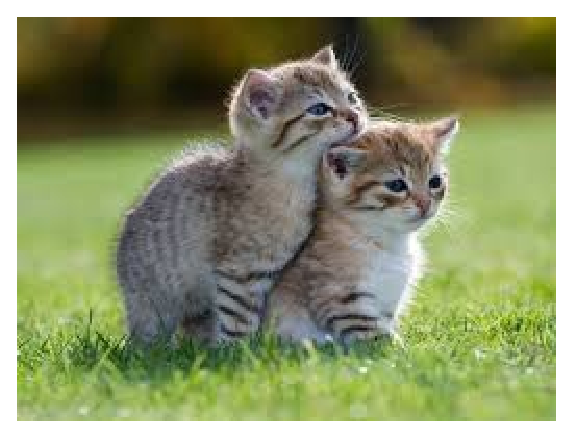
\includegraphics[width = 0.5\textwidth]{figuras/resultados/joy_hand_control}
\caption{Imagem do controle da cadeira de rodas}
\label{fig:joy_hand_control}
\end{figure}

O \textit{joystick} utilizado é composto por dois potenciômetros que indicam as posições em dois eixos independentes. Utilizando os potenciômetros como simples divisores de tensão é possível inferir as posições de seus eixos a partir da medições das tensões do circuito, para realizar esta medição e então rastrear o comando de movimento do usuário, são utilizados dois canais de conversores AD para os potenciômetros, tais conversores são internos ao microcontrolador utilizado e não necessitam de nenhum \textit{hardware} extra.

A rotina de trabalho do microcontrolador do módulo Joystick consiste em adquirir os valores analógicos das posições do \textit{joystick}, convertê-los em valores digitais de um \textit{byte} cada, diferenciando-os utilizando a estratégia de representar um eixo apenas por valores ímpares e o outro apenas por valores pares (ambos entre 0 e 255) e enviá-los via serial alternadamente em um laço infinito, conforme a figura \ref{fig:joy_fluxogram}.

\begin{figure}[!htb]
\centering
\includegraphics[width = 0.9\textwidth]{figuras/resultados/joy_fluxogram}
\caption{Rotina de trabalho do microcontrolador do módulo Joystick}
\label{fig:joy_fluxogram}
\end{figure}

\begin{comment}

Joystick
  - Software e Hardware (periféricos e MSP Joystick)
    - Colocar imagem de código
  - Interface de usuário
    - Fotos do controle

\end{comment}

\subsection{Controlador Central}

  O Raspberry será utilizado como central de comandos para processar as informações vindas do MSP dedicado ao módulo Joystick e enviar o resultado deste processamento para o MSP dedicado aos Motores.

  \textbf{Comunição entre MSP e Raspberry}

  A comunicação, tanto entre o MSP do Josytick e o Raspberry, quanto entre o MSP do Motor e o Raspberry, estão sendo feitas via \textit{threads}.

  A conexão entre os MSP foi formulada através do método \textit{findPort}. Sua implementação pode ser observada na figura \ref{fig:find_port_method}.

  \begin{figure}[!htb]
    \centering
    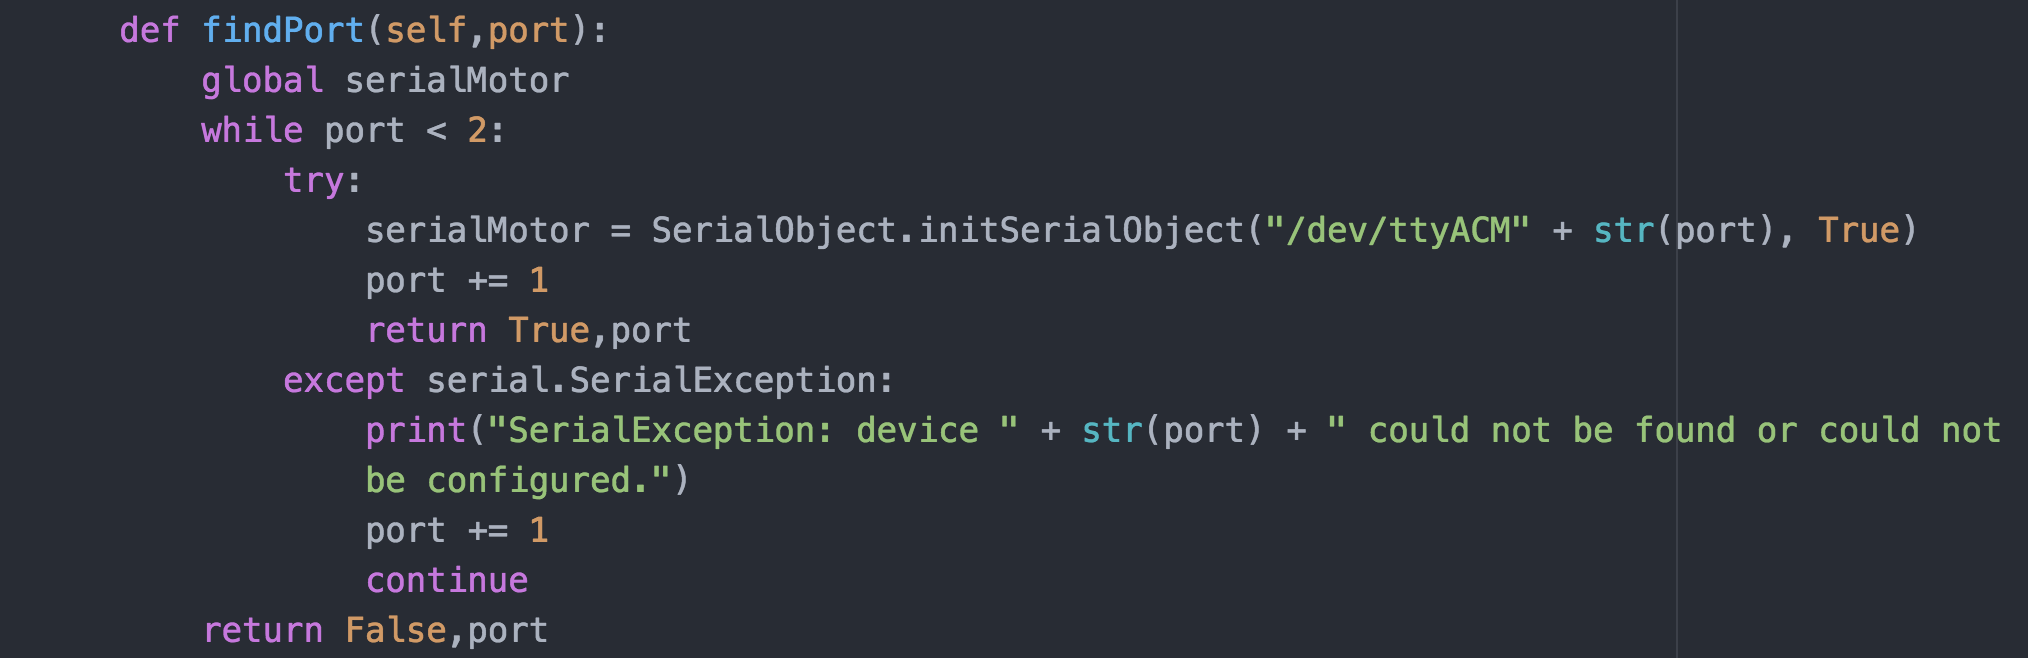
\includegraphics[width=0.9\textwidth]{figuras/resultados/find_port_method}
    \caption{Método para encontrar porta dinamicamente}
    \label{fig:find_port_method}
  \end{figure}

  Este método permite que tanto o MSP do Joystick quanto o MSP do Motor, sejam conectados sem a previa identificação de qual porta utilizar para comunicação. Porém, há existência de prioridade entre as \textit{threads}, ou seja, enquanto a \textit{threads} do Joystick não se conectar com sucesso a \textit{threads} do Motor não irá se conectar.

  Para que este processo ocorra com sucesso, uma checagem de dados é feita para cada tentativa de conexão. Esta checagem consiste em verificar se a porta, a ser conectada, está enviando dados ou recebendo. Para que a conexão do Josytick ocorra com sucesso, a porta deva estar recebendo dados, para que a conexão do Motor ocorra com sucesso, a porta não deve enviar dados. A implementação desta checagem pode ser verificada na figura \ref{fig:try_receive_data}.

  \begin{figure}[!htb]
  \centering
  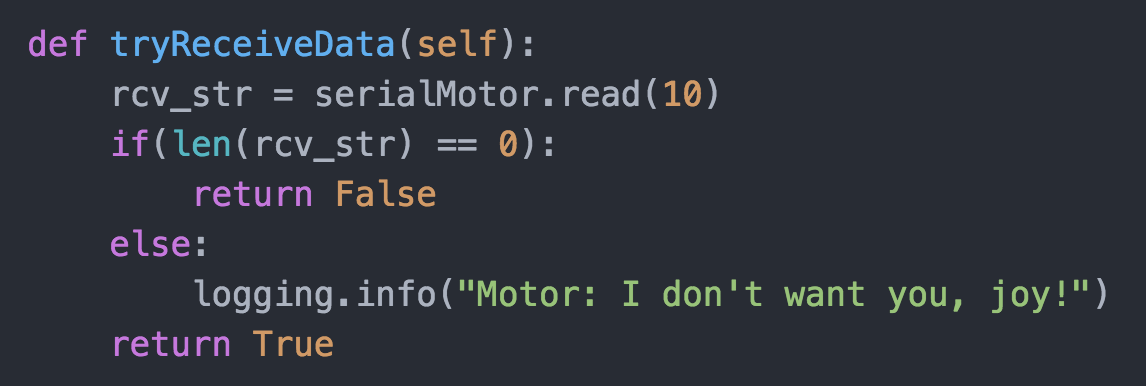
\includegraphics[keepaspectratio=true,scale=0.5]{figuras/resultados/try_receive_data}
  \caption{Método para checar se existe recebimento de dados em porta. Caso do Motor.}
  \label{fig:try_receive_data}
  \end{figure}

  Esta estratégia auxilia na manutenção do produto, pois caso algum MSP fique inutilizavel, é possivel colocar outro MSP, previamente configurado, no lugar do componente inutilizado.

  Após o Raspberry conseguir encontrar uma porta para se conectar com o MSP do Joystick, então a \textit{thread} do MSP do Motor utiliza do mesmo método para se conectar.

  Ao se ter as duas conexões estabelecidas, então o recebimento de dados são adquiridos do Joystick e enviados para os Motores. Para se fazer este envio de informações de forma correta é necessário fazer a sincronização entre as \textit{threads}.

  \textbf{Sincronização de \textit{Threads}}

  Foi percebido que as \textit{threads} precisam estar sincronizadas para se fazer o envio de informações de forma correta. Pois a \textit{thread} do Joystick recebe as informações, e a \textit{thread} do Motor consome estas informações.

  Este problema de sincronização das \textit{threads} é conhecido como um clássico problema de \textit{threads}: Produtor e Consumidor.

  Este problema é caracterizado por 2 processo que compartilharem de um \textit{buffer} comum, no qual o produtor insere a informação no \textit{buffer} e o consumidor retira a informação do \textit{buffer}. Possíveis problemas: Produtor insere produto onde não foi consumido e consumidor remove informação onde já foi removido. Mais detalhes do problema no capítulo \ref{cap:fundamentacao_teorica}.

  Este problema foi solucionado com os seguintes passos:
  \begin{enumerate}
    \item Produtor: Produz os itens necessários em \textit{buffer}, no caso os valores referentes aos potenciometros do Joystick. Neste momento a \textit{thread} do Consumidor é parada e uma variável responsável por esta trava é notificada. Isto pode ser visto na figura \ref{fig:joy_lock};
    \item Consumidor: Consume os itens em \textit{buffer} enviado os mesmos para o MSP dos Motores. Neste momento a \textit{thread} do Produtor é parada e a variável responsável pela trava é consumida. Isto pode ser visto na figura \ref{fig:motor_lock};
  \end{enumerate}

  A variável de trava é utilizada com o propósito de se fazer a produção e o consumo de forma sincronizada. O processo do Consumidor somente será ativo quando o processo do Produtor setar a variável de trava.

  \begin{figure}[!htb]
  \centering
  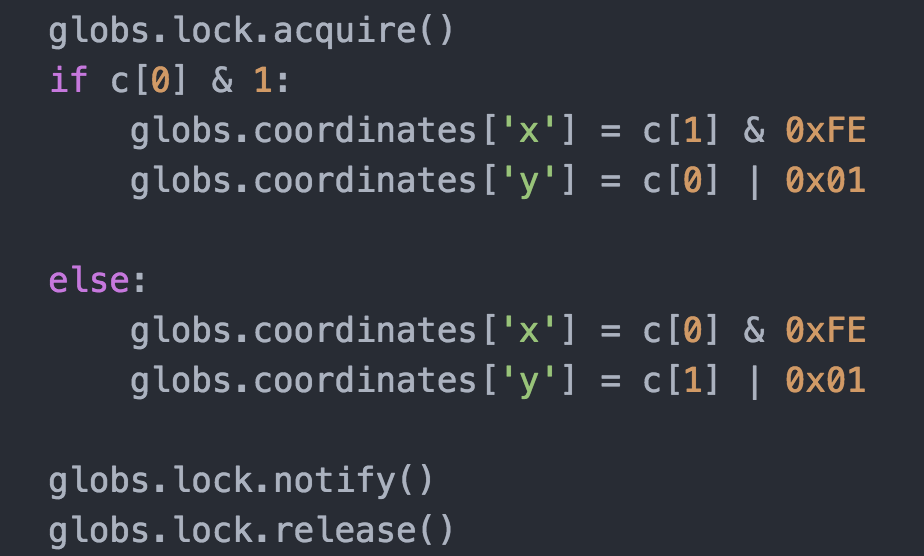
\includegraphics[keepaspectratio=true,scale=0.5]{figuras/resultados/joy_lock}
  \caption{Código utilizado para notificar variável de trava}
  \label{fig:joy_lock}
  \end{figure}

  \begin{figure}[!htb]
  \centering
  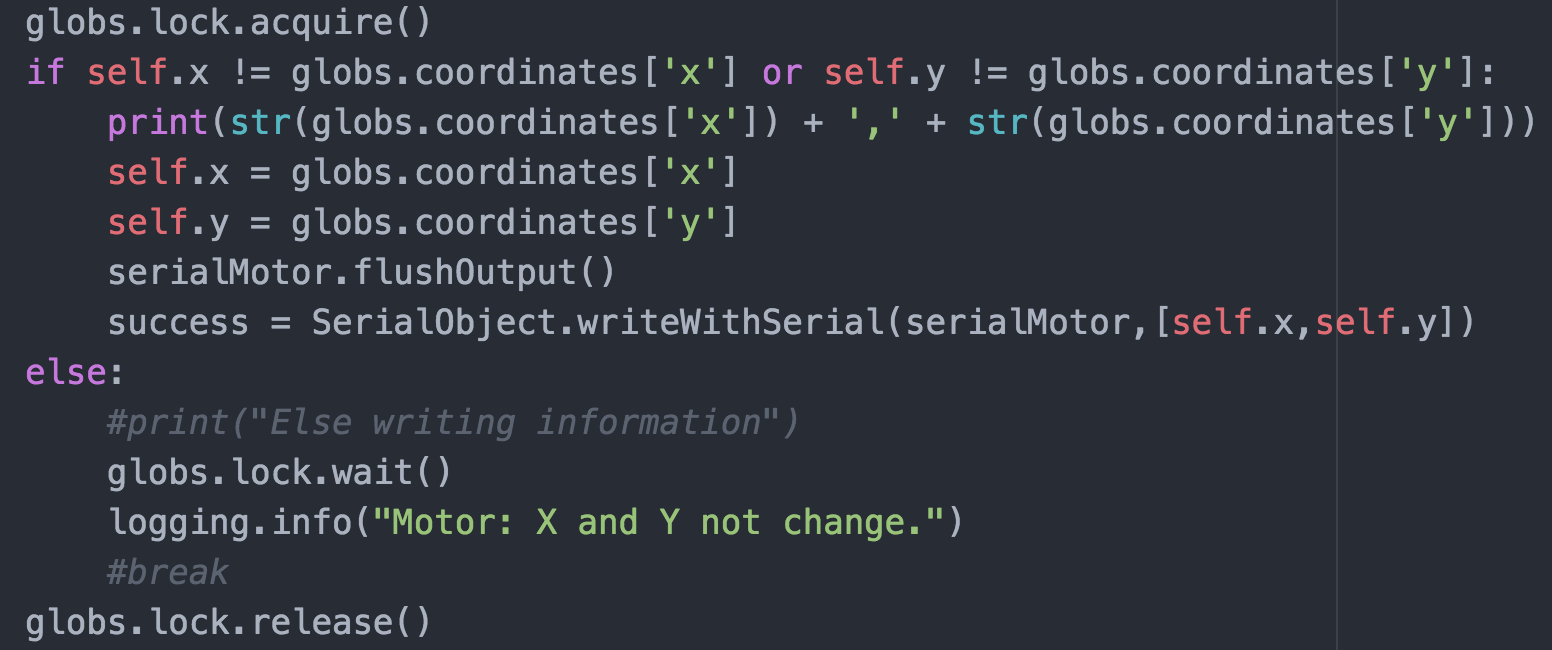
\includegraphics[width=0.9\textwidth]{figuras/resultados/motor_lock}
  \caption{Código utilizado para consumir itens e consequentemente a variável de trava}
  \label{fig:motor_lock}
  \end{figure}

\subsection{Motor}

    O modulo Motor é utilizado para fazer a movimentação da cadeira, conforme os comandos enviados pelo usuário através do módulo Joystick. O módulo Motor é composto por 2 motores de corrente contínua e um microcontrolador.

    O microcontrolador deste módulo tem como intuito receber as informações do controlador central e gerar 2 pulsos de PWM, um para cada motor. As funções \textit{update\_left} e \textit{update\_right}, vide figura \ref{fig:update_motors}, tem como objetivo atualizar o \textit{duty cycle} para cada motor.

    \begin{figure}[!htb]
    \centering
    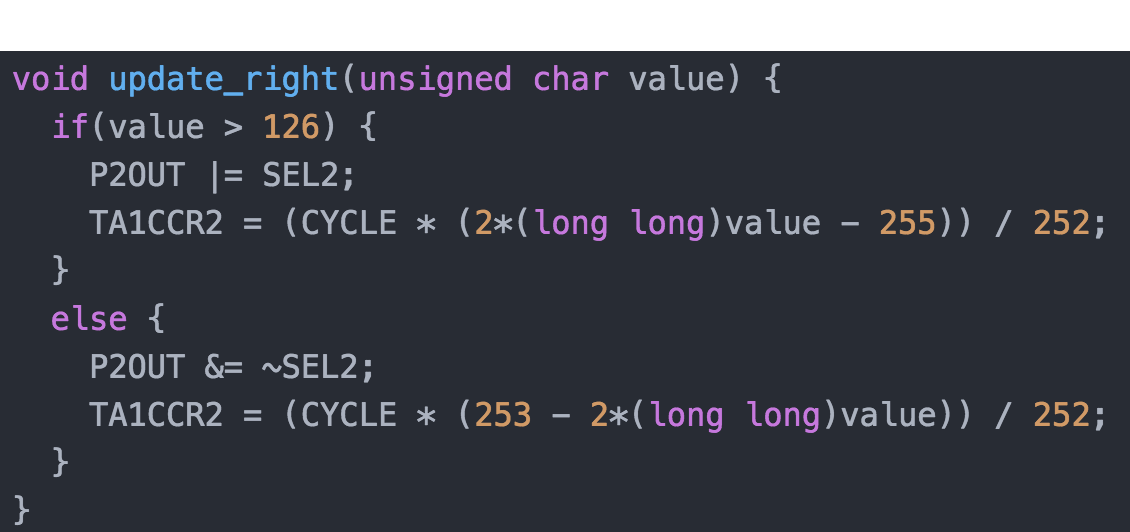
\includegraphics[width = 0.5\textwidth]{figuras/resultados/update_motor_right}
    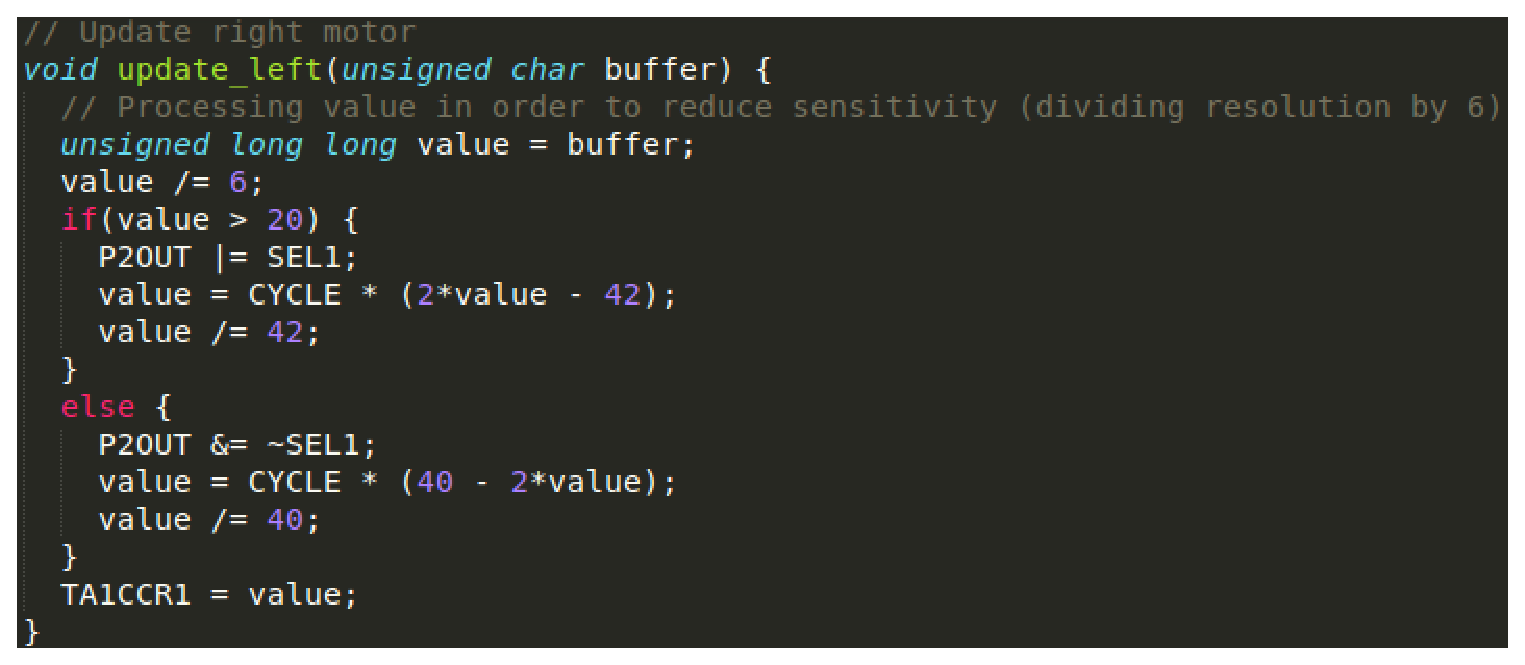
\includegraphics[width = 0.5\textwidth]{figuras/resultados/update_motor_left}
    \caption{Funções para atualização de taxa do \textit{duty cycle}}
    \label{fig:update_motors}
    \end{figure}

    Os valores são recebidos através da função \textit{update}, vide figura \ref{fig:update}, responsável por receber de forma correta os dados. Esta rotina consiste em verificar se o valor recebido é impar ou par. Isto é feito por causa da estratégia utilizada para diferenciar os dados de cada potenciômetro enviados do módulo Joystick, através do controlador central.

    \begin{figure}[!htb]
    \centering
    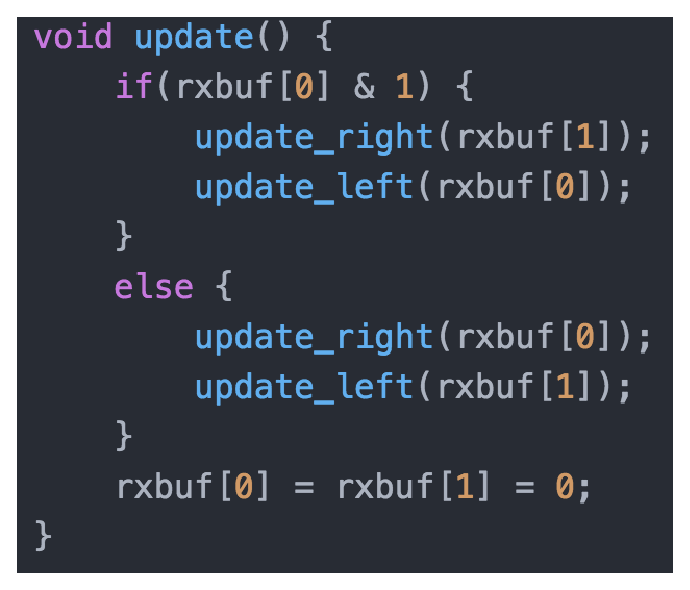
\includegraphics[width = 0.5\textwidth]{figuras/resultados/update}
    \caption{Função para diferenciação de dado recebido}
    \label{fig:update}
    \end{figure}


    A função \textit{update\_left} recebe os valores pares, e a função \textit{update\_right} recebe os valores impares.

\subsection{Integração Motor e Joystick}

Para se fazer a movimentação da cadeira de forma correta, foi feito um mapeamento dos possíveis estados de movimentação. Estes estados foram inicialmente mapeados utilizando os valores do módulo do Joystick. Com base nos estados mapeados, a intensidade e direção dos motores são formulados. Esta integração foi implementada na Raspberry.

  \textbf{Mapeamento dos Estados em Relação ao Joystick}

  Estes estados, vide tabela \ref{tab:tabela-pots}, são formalizados a partir das possibilidades de valores que podem ser capturados do módulo Joystick.

  Os valores do potenciômetro 1 são referenciados para o motor da esquerda e os valores do potenciômetro 2 são referenciados para o motor da direita.

  \begin{table}[!ht]
  \centering
  \resizebox{\textwidth}{!}{%
  \begin{tabular}{|c|c|c|c|}
  \hline
  ID & Valor Potenciômetro 1  & Valor Potenciômetro 2  & Estado \\ \hline
  1 & 254 & 255 & Para frente \\ \hline
  2 & 254 & 1 & Virar para direita (próprio eixo) \\ \hline
  3 & 254 & 127 & Virar para direita (eixo motor 2) frontal \\ \hline
  4 & 126 & 127 & Parado \\ \hline
  5 & 126 & 255 & virar para esquerda (eixo motor 1) frontal \\ \hline
  6 & 126 & 1 & virar para esquerda (eixo motor 1) traseiro \\ \hline
  7 & 0 & 1 & Para trás \\ \hline
  8 & 0 & 255 & Virar para esquerda (próprio eixo) \\ \hline
  9 & 0 & 127 & virar para direita (eixo motor 2) traseiro \\ \hline
  \end{tabular}
  }
  \caption{Mapeamento dos estados conforme valores do Joystick}
  \label{tab:tabela-pots}
  \end{table}

  Para elucidar os estados da tabela \ref{tab:tabela-pots} a figura \ref{fig:estados} foi confeccionada.

  \begin{figure}[!ht]
    \center
    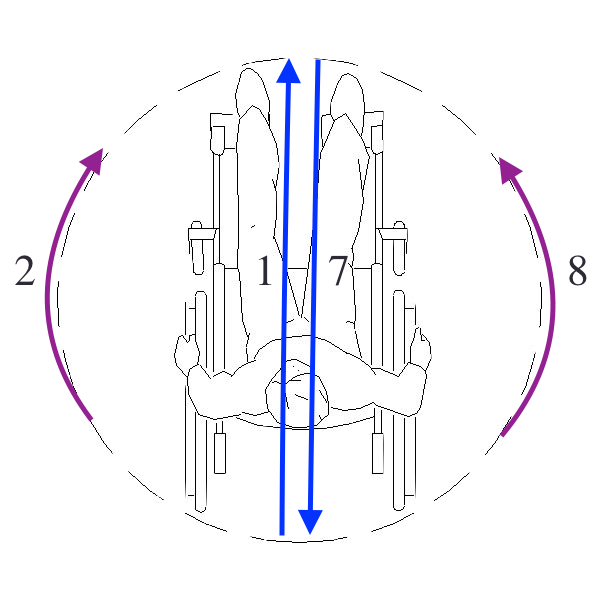
\includegraphics[width=0.3\textwidth]{figuras/resultados/estados_1_2_7_8}
    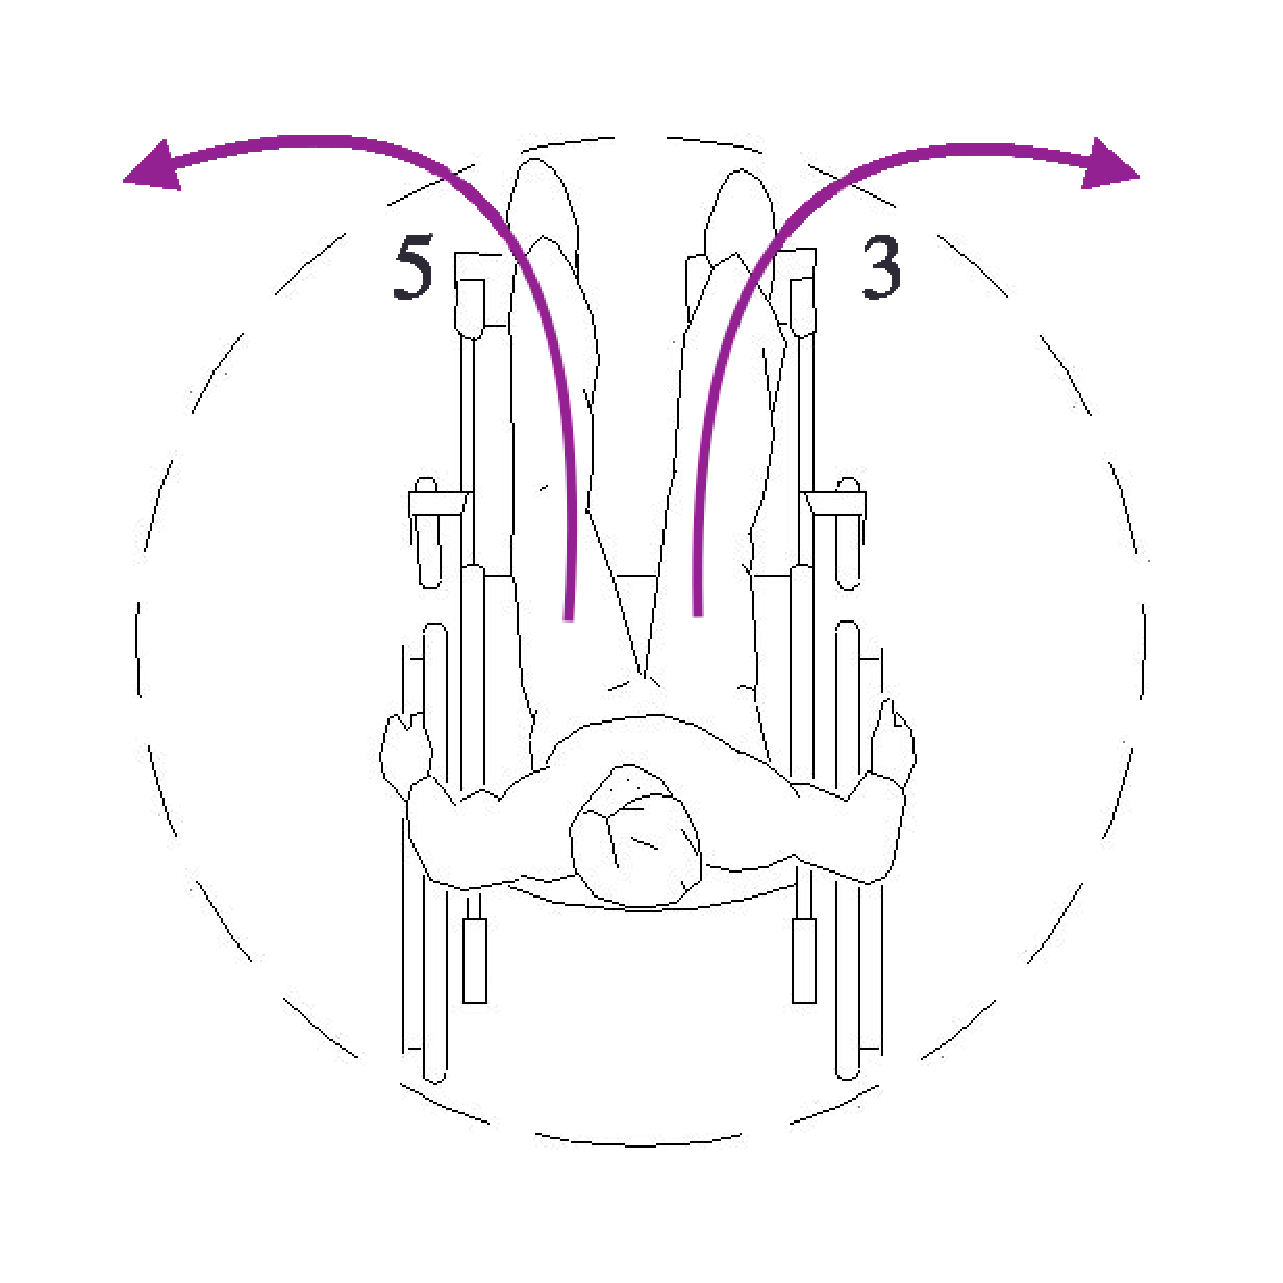
\includegraphics[width=0.3\textwidth]{figuras/resultados/estados_3_5}
    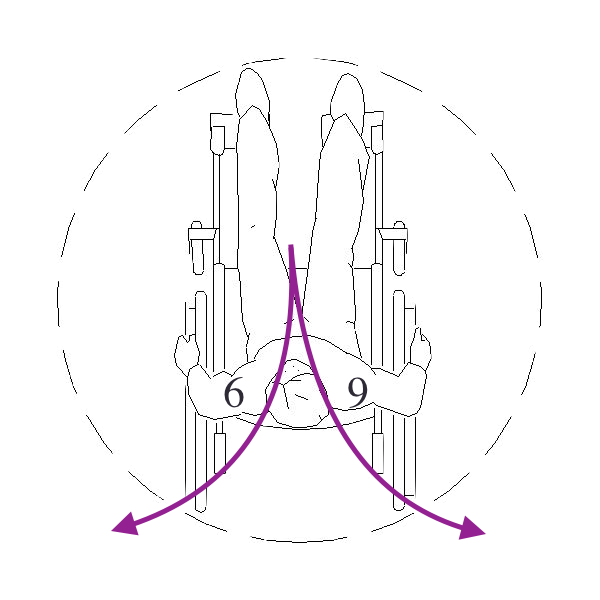
\includegraphics[width=0.3\textwidth]{figuras/resultados/estados_6_9}
    \caption{Estados da cadeira}
    \label{fig:estados}
  \end{figure}

  \textbf{Mapeamento de Intensidade e Direção dos Motores}

    Conforme os estados mapeados na tabela \ref{tab:tabela-pots}, as intensidades e direções de cada motor são definidas na tabela \ref{tab:tabela-pots2}.

    \begin{table}[!ht]
    \centering
    \resizebox{\textwidth}{!}{%
    \begin{tabular}{|c|c|c|c|}
    \hline
    ID & Estado & Motor 1(Intensidade(\%), Direção) & Motor 2(Intensidade (\%), Direção) \\ \hline
    1 & Para frente & (100, + ) & (100, + ) \\ \hline
    2 & Virar para direita (próprio eixo) & (100, +) & (100, -) \\ \hline
    3 & Virar para direita (eixo motor 2) frontal & (100, +) & (0 , *) \\ \hline
    4 & Parado & (0, *) & (0, *) \\ \hline
    5 & Virar para esquerda (eixo motor 1) frontal & (0, *) & (100, +) \\ \hline
    6 & Virar para esquerda (eixo motor 1) traseiro & (0, *) & (100, -) \\ \hline
    7 & Para trás & (100, -) & (100, -) \\ \hline
    8 & Virar para esquerda (próprio eixo) & (100, -) & (100, +) \\ \hline
    9 & Virar para direita (eixo motor 2) traseiro & (100, -) & (0, *) \\ \hline
    \end{tabular}
    }
    \caption{Intensidade e direção dos motores conforme estado. Asteriscos simbolizam motor sem direção}
    \label{tab:tabela-pots2}
    \end{table}

    \textbf{Integração de \textit{joystick}}

    O hardware utilizado no módulo Joystick, vide capítulo \ref{cap:fundamentacao_teorica}, para fazer o controle da cadeira, foi acoplado usando uma rotação de 45 graus no sentido anti-horário. Isto foi feito para melhorar a interpretação dos dados. Esta translação do eixo XY dos potenciômetros do \textit{joystick}, vide figura \ref{fig:joy_superior}, para o novo eixo M1M2, vide figura \ref{fig:joy_m1m2}, nos permite inserir os estados da tabela \ref{tab:tabela-pots} e implementar estes estados de forma mais fácil.

    \begin{figure}[!ht]
      \center
      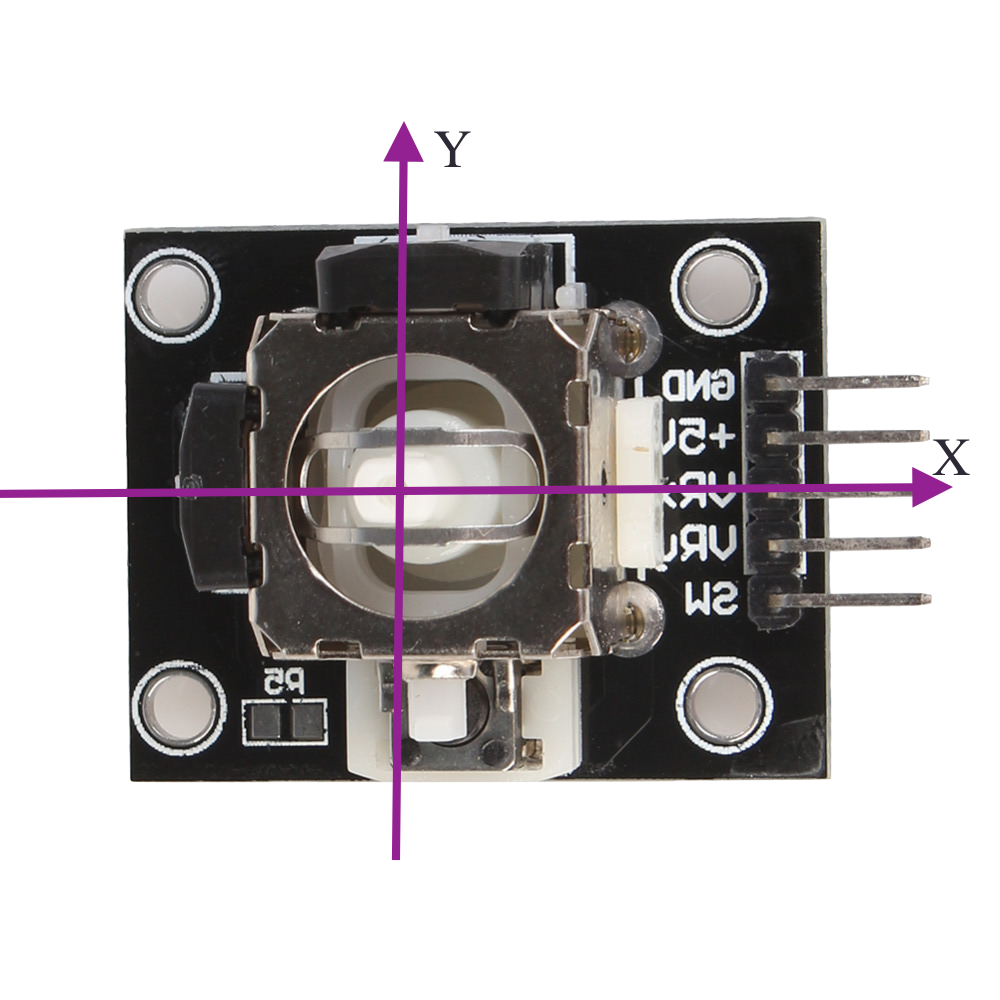
\includegraphics[width=0.4\textwidth]{figuras/resultados/joy_xy}
      \caption{Visão de \textit{joystick} com eixos para propósito geral}
      \label{fig:joy_superior}
    \end{figure}

    \begin{figure}[!ht]
      \center
      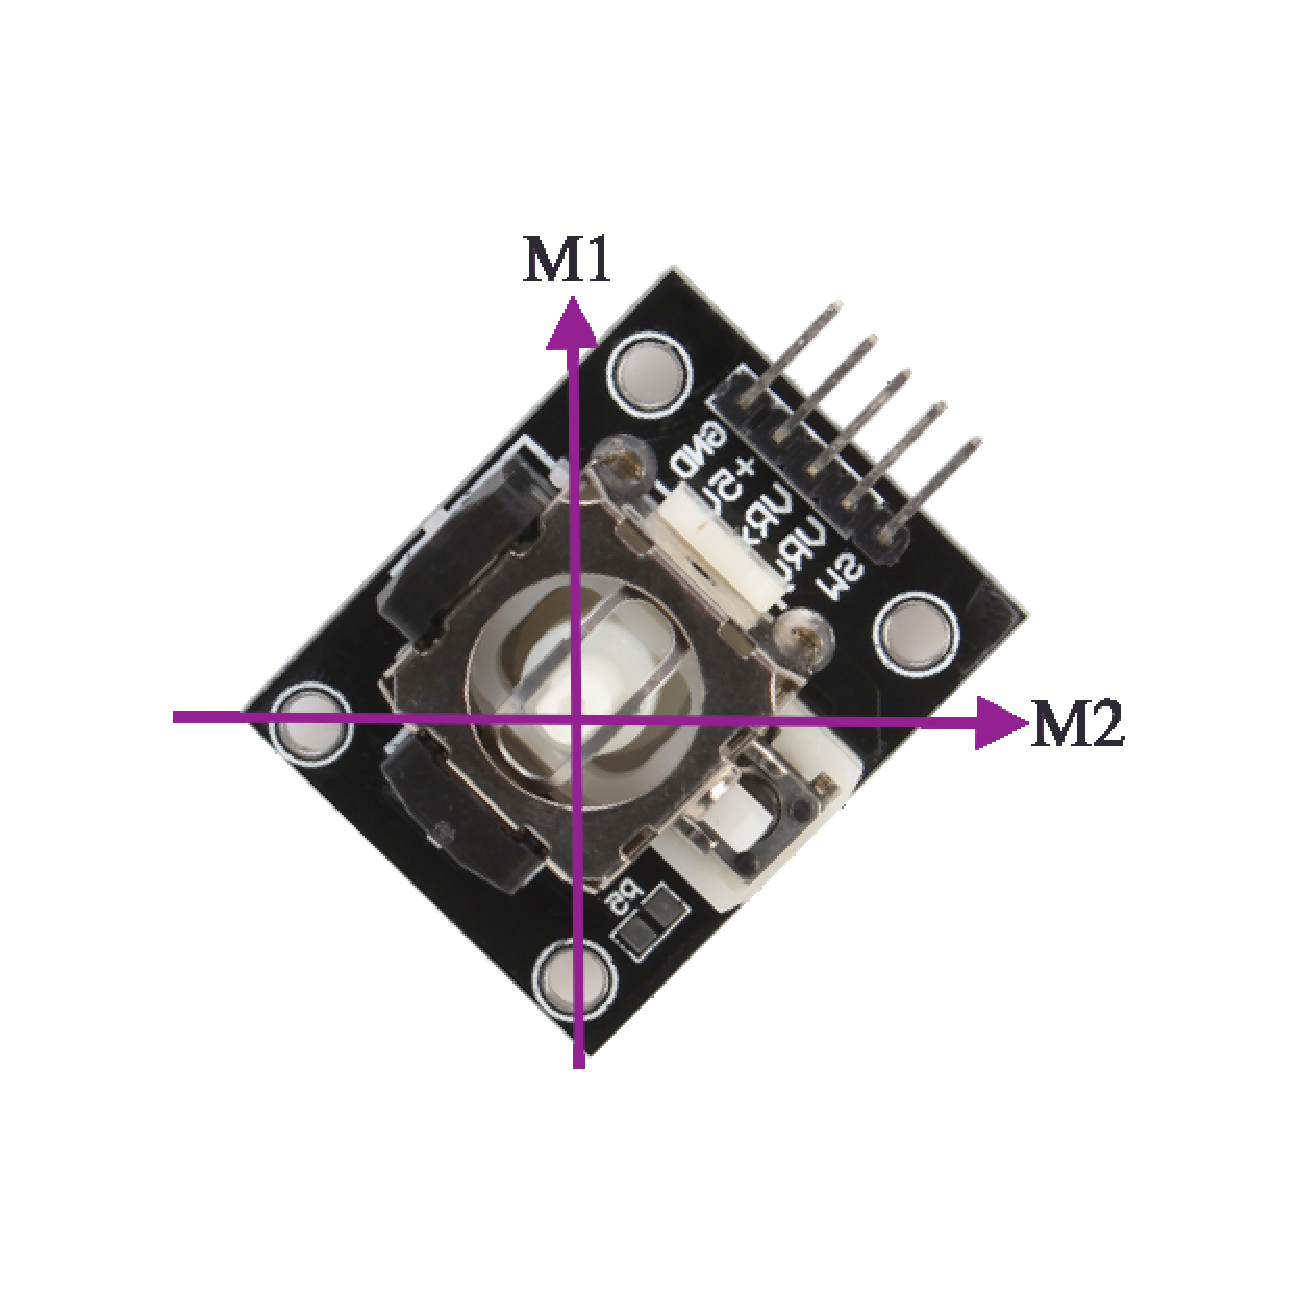
\includegraphics[width=0.5\textwidth]{figuras/resultados/joy_m1m2}
      \caption{Visão de \textit{joystick} com eixos rotacionados}
      \label{fig:joy_m1m2}
    \end{figure}



\begin{comment}

Integração Motor e Joystick
#  - Mapeamento dos estados em relação ao joystick (255,255->Frente)
#  - Mapeamento dos estados em relação aos motores (intensidade, direção)
  - Integração via software ou via hardware
    - Soft
      Vantagens: Uso de propósito geral
      Desvantagem: capacidade de Processamento para cálculo de transformação
    - Hardware:
      Vantagens: Valores de intensidade e direção dos motores são adquiridos de forma instanea
      Desvantagem: Não foi observados desvantagens para a aplicação, porém para outros propósitos é mais dificil de se utilizar os dados, pois os mesmos não tem uma relação direta com o plano cartesiano original.

Ponte-H (copiar e colar do documento pc2)
  - Circuito de direcionamento das PWMs através das seletoras (demultiplexador)

Alimentação do sistema
  - Esquema de alimentação do sistema
  - Circuito regulador de tensão
\end{comment}

\subsection{Ponte H}

No decorrer da produção do circuito da ponte H, foi utilizado uma porta NAND e duas porta AND para garantir que não haverá acionamento de todos os transistores ao mesmo tempo.

Foi necessário utilizar um dobrador de tensão no circuito, com ele foi possível garantir um VGS maior que 2V para polarização dos transistores MOSFET da ponte. Como a alimentação da ponte está restrita nos 12V teve-se que utilizar esse artificio para conseguir criar essa diferença de tensão nos terminais do transistor e polariza-lo.

O circuito do dobrador, representado na figura \ref{fig:figx+4}, possui um oscilador que gera uma onda quadrada, que no caso é um CI 555, e para o controle do pulso temos os resistores R5 e R6 e o capacitor C4. Em C2 tem-se um capacitor inversamente polarizado o que faz com que esse carregue apenas quando a parte baixa da onda quadrada é ativada.

Durante o período da onda quadrada em alto, C3 descarrega na saída do diodo na parte negativa gerando um efeito que dobra a tensão, conforme pode ser visto na figura \ref{fig:figx+4}. É importante observar que o capacitor C2 não pode ser muito grande e nem o pulso do oscilador muito largo para que não haja uma descontinuidade muito grande no valor de tensão.

Esse circuito é necessário pois a tensão do circuito está limitada em 12V. Com isso não é possível conseguir um VGS maior que 2V nos transistores MOSFET da ponte H. Com o auxílio desse artifício muito utilizado na eletrônica consegue-se fazer a transformação de um tensão DC em uma tensão DC com o dobro de tensão, com isso tem-se 24V teóricos na saída do circuito dobrador de tensão, pois a tensão de entrada é cerca de 12V.

Dessa forma liga-se a saída do dobrador de tensão nos transistores Q7 e Q8 para eles alimentarem o Gate dos transistores MOSFET do circuito, como há perdas envolvidas, chegarão cerca de 22V nas portas G dos transistores, tornando possível haver uma diferença maior que a VTH e polarizando os transistores da maneira correta e permitindo o funcionamento do sistema por completo.

\begin{figure}[!htb]
	\centering
	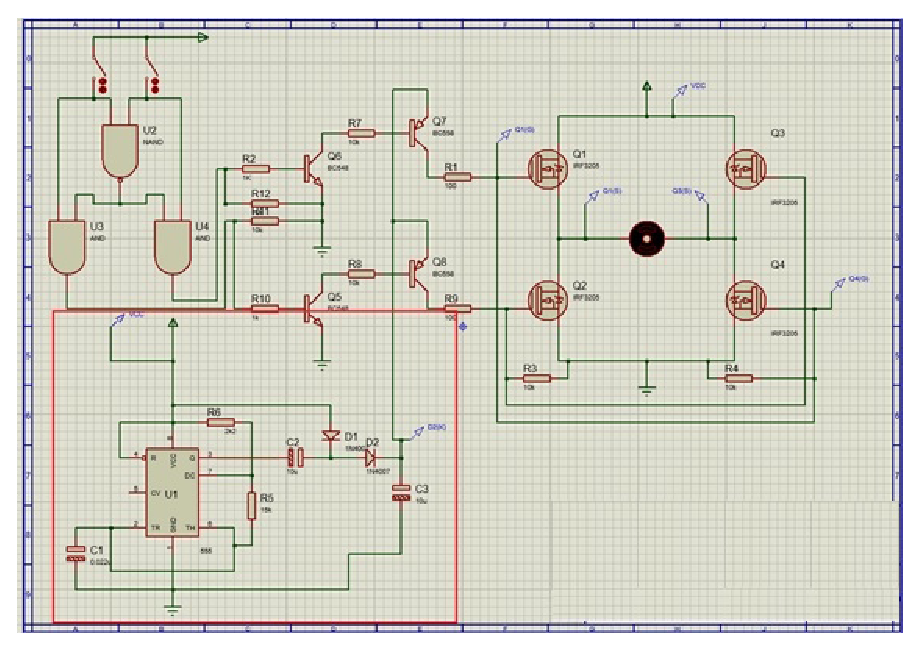
\includegraphics[keepaspectratio=true,scale=0.8]{figuras/referencialteorico/figurax_4.eps}
	\caption{Circuito elevador te tensão}
	\label{fig:figx+4}
\end{figure}


Para facilitar e proteger o sistema, será construído um distribuidor que vai ser basicamente uma placa que facilitará a conexão de todos os outros módulos ao sistema, assim não será necessário que haja reduções de tensão tão drásticas nos módulos, pois essa já estará pronta no distribuidor.

O distribuidor vai ser responsável por alimentar os motores elétricos e os módulos de controle dos movimentos da cadeira de rodas. Ele contará com um bloco de entrada que estará conectado diretamente nos terminais da bateria, onde a partir desse bloco de entrada teremos duas saídas de distribuição, uma com 12 volts e outra com 5 volts.

A saída de distribuição de 12 volts será realizada através de cabos que serão conectados nos terminais dos motores. Essa saída será dupla, ou seja, cada motor terá sua alimentação individual, sendo que para proteção dos dois motores, utilizaremos fuzíveis inseridos antes dos plugs dos moteres, para que caso ocorra alguma variação de corrente, os motores não sejam danificados.

A saída de distribuição de 5 volts será proveniente da utilização de um regulador de tensão 7805. Serão utilizados diodos zeners(falar qual) que garantirão que a tensão se mantenha estável nos 5 volts. Essa saída será responsável pela alimentação das duas pontes H, da Raspberry Pi, dos 3 msp430 e do joystick.

Esse distribuidor de tensão pode ser visto no diagrama apresentado na figura \ref{fig:diagrama_controle}.

\begin{figure}[!htb]
	\centering
	\includegraphics[keepaspectratio=true,scale=0.4]{figuras/resultados/fluxograma}
	\caption{Diagrama do sistema de controle}
	\label{fig:diagrama_controle}
\end{figure}

Foram feitas duas versões de ponte H. Na primeira versão da ponte H utilizava-se trilhas com cerca de 5 mm para os motores e transistores. Após alguns testes foi verificado que a espessura não suportava a corrente que os motores necessitam, as trilhas estavam soltando da placa.

Com isso foi necessário reestruturar a ponte H, então foi idealizado o paralelo de 2 pontes H para alimentar cada motor. Para testar o paralelo foi necessário conhecer a corrente que cada ponte estava puxando. Segundo as especificações do motor, a corrente que cada motor puxa é de 25A. Em teoria cada ponte em paralelo deveria estar com no máximo 12,5A em sua saída, porém a aferição dessa corrente é complexa, pois não tinha-se instrumento de medida que suportasse tamanha corrente. Dessa forma desenvolveu-se um sistema de medida usando a proteção contra sobre-corrente do sistema, que é constituída de fusíveis automotivos de 12V. Variando os fusíveis de 5A em 5A e esperando eles se romperem, teve-se uma estimativa que sem carga o sistema estava puxando entre 10 e 15A.

Após alguns testes, verificou-se que as trilhas continuavam não suportando a corrente quando colocava-se carga. Para solucionar o problema, foi montado um novo esquemático com as trilhas de grandes espessuras, 3,5cm, como na figura \ref{fig:novo_esquematico_ponte_h} para auxiliar na dissipação de calor do sistema. Usando os mesmo transistores, porém fora da placa e fixados diretamente no dissipador, mas com as ligações feitas através de cabos externos como mostrado na figura \ref{fig:ponte_h_dissipador}.

\begin{figure}[!ht]
  \center
  \includegraphics[width=0.6\textwidth]{figuras/resultados/ponte_h_dissipador}
  \caption{Ponte H e dissipador}
  \label{fig:ponte_h_dissipador}
\end{figure}


O circuito de controle foi mantido similar ao primeiro layout e foi feito algumas pequenas modificações na proteção da entrada do sinal do PWM do circuito para garantir que não haverá curto circuito no sistema.

As novas trilhas suportariam a corrente, contudo era necessário soldar o transistor, foi usado então fios para conectar os transistores a ponte H e ligados como mostrado na figura \ref{fig:novo_esquematico_ponte_h}. Cada um dos quatro transistores, possui um Gate, que é um pino de controle, o Drain, que é a saída do transistor e o Source, que é a entrada. Foram enumeradas entradas e saídas com os respectivos transistores, onde 1d equivale ao transistor 1 pino de Drain, 1s ao transistor 1, pino de Source e assim por diante. O pino de controle foi ligado direto a antiga formação da ponte H, já que essa possuía os devidos circuitos de ativar a ponte H e proteger os pinos de controle, usados no PWM.

\begin{figure}[!ht]
  \center
  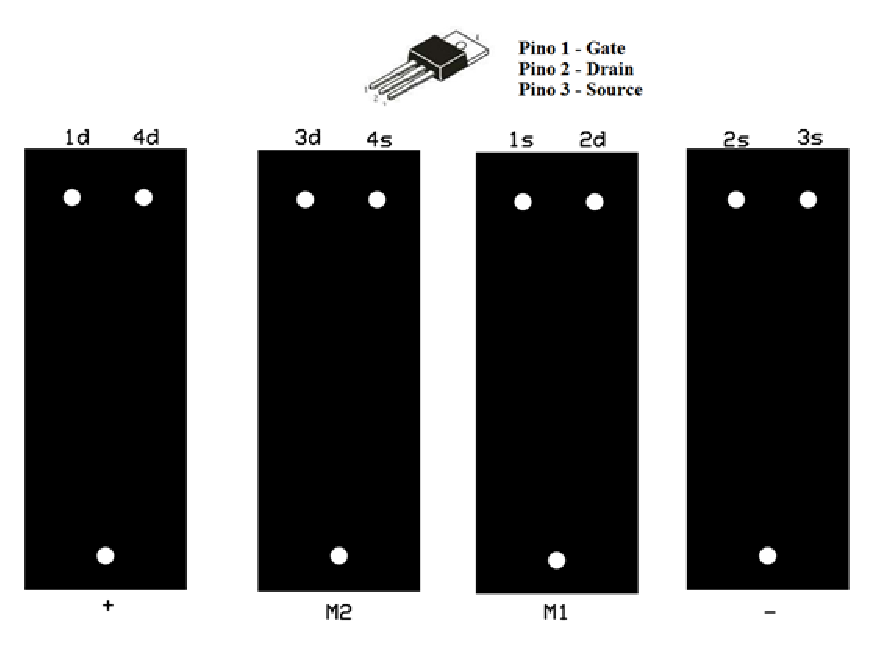
\includegraphics[width=0.7\textwidth]{figuras/resultados/novo_esquematico_ponte_h}
  \caption{Novo esquemático ponte H}
  \label{fig:novo_esquematico_ponte_h}
\end{figure}


\subsection{Dissipador de calor}

Os circuitos de potência modernos possuem elevado rendimento, porém a quantidade de
calor gerada é uma preocupação. Atualmente os dispositivos operam com potências elevadas
e no limite da capacidade de dissipação. O uso de um dissipador é tão importante quanto à
parte elétrica do circuito.

O objetivo dessa sessão é fornecer subsídios para estabelecer critérios para o
dimensionamento do sistema de dissipação do calor produzido por componentes eletrônicos,
especialmente semicondutores de potência da ponte H(transistores), buscando a proteção de
tais componentes.

Considerando:

$P_t$ = Potência a ser dissipada pelo transistor;

$T_j$ = Temperatura de junção;

$T_c$ = Temperatura de carcaça;

$T_{amb}$ = Temperatura ambiente;

$R_{jc}$ = Resistência térmica na junção $[\frac{{\circ}\mathrm{C}}{W}]$;

$R_{ch}$ = Resistência térmica na carcaça $[\frac{{\circ}\mathrm{C}}{W}]$;

$R_{ha}$ = Resistência térmica dissipador - ambiente $[\frac{{\circ}\mathrm{C}}{W}]$;

Onde $T_j$ e $R_{jc}$ são parãmetros do \textit{Datasheet}. Foram utilizadas duas ponte H, sendo
que cada uma possui 4 transistores IRF3205(Jameco Part Number 618089)\cite{jameco}:

$T_j = -55 à 175\,^{\circ}\mathrm{C}$;

$R_{jc} = 0,75[\frac{{\circ}\mathrm{C}}{W}]$;

$R_{ch} = 0,5[\frac{{\circ}\mathrm{C}}{W}]$;

Assim podemos calcular $R_{ha}$ como:

\begin{equation}
 R_{ha} = \frac{(T_j - T_{amb})}{P_t} - R_{jc} + R_{ch}
\end{equation}

A potência total dissipada é de 300W por cada ponte H, assim cada transistor recebe 75W. A
temperatura ambiente considerada é de $T_j$ como $40\,^{\circ}\mathrm{C}$, considerando a $T_j$ como $130\,^{\circ}\mathrm{C}$,
temos assim:

\begin{equation}
 R_{ha} = \frac{(130 - 40)}{300} - 0,75 + 0,5 = 0,05\,\frac{^{\circ}\mathrm{C}}{{W}}
\end{equation}

Superfícies aletas, chamadas de dissipadores de calor são
comumente utilizadas para o resfriamento de dispositivos eletrônicos. A energia dissipada por
esses dispositivos é transferida por condução dos dispositivos de potência para os dissipadores
e por convecção natural ou forçada dos dissipadores para o ambiente \cite[p.~434-439]{cengel}.

Uma das principais questões na escolha de um dissipador de calor é escolher entre um com
aletas estreitamente espaçadas ou aletas amplamente espaçadas para uma determinada área
da base. Um dissipador com menor espaçamento entre as aletas terá maior superfície de
transferência de calor, mas o coeficiente de transferência de calor é menor devido a
resistência que as aletas introduzem no fluxo do ar.

\subsection{Indicador de Nível de Bateria}

É importante saber o nível de bateria da cadeira de rodas, com isso é possível controlar sua autonomia e saber quando ela irá parar de funcionar. O indicador servirá para informar quando a bateria estiver acabando, para que se possa voltar para estação de recarga e recarregar a cadeira de rodas.

Será utilizado um multimetro automotivo de bateria como mostrado na figura \ref{fig:indicador_bateria}. Eles são comumente utilizados para medir as baterias auxiliares utilizadas em sons automotivos. Seu funcionamento baseia-se na medição da diferença de tensão nos polos da bateria, dessa forma indicando qual é a tensão da bateria. Quando a tensão cair a um nível crítico é quando os motores da cadeira de rodas irão parar de funcionar, no caso do motor do projeto, 9V. Quando o indicador chegar em 9V, o usuário deve retornar com a cadeira de rodas para que a mesma seja recarregada.

\begin{figure}[!ht]
  \center
  \includegraphics[width=0.7\textwidth]{figuras/resultados/indicador_bateria}
  \caption{Multimetro automotivo de bateria}
  \label{fig:indicador_bateria}
\end{figure}
